\documentclass[10pt]{article}
\usepackage[margin=0.62in]{geometry}
\usepackage{graphicx}
\usepackage{booktabs}
\usepackage{float}
\usepackage{hyperref}
\usepackage{xcolor}
\usepackage{enumitem}
\usepackage{subcaption}
\usepackage{titlesec}

\hypersetup{colorlinks=true, linkcolor=blue, urlcolor=blue, citecolor=blue}
\setlength{\parskip}{0.2em}
\setlength{\parindent}{0pt}
\setlist[itemize]{leftmargin=1em, topsep=1pt, itemsep=1pt, parsep=0pt}
\setlength{\textfloatsep}{4pt}
\setlength{\floatsep}{3pt}
\setlength{\intextsep}{3pt}
\setlength{\abovecaptionskip}{2pt}
\setlength{\belowcaptionskip}{0pt}
\captionsetup{font=small, skip=2pt}
\captionsetup[subfigure]{font=scriptsize, skip=1pt}
\titlespacing*{\section}{0pt}{5pt}{2pt}
\renewcommand{\arraystretch}{0.95}
\setlength{\tabcolsep}{5pt}
\graphicspath{{report_figures/}}

\title{\vspace{-1.0em}An Empirical Study of Different Optimizers Across Different Tasks\vspace{-0.6em}}
\author{Ananya Jha \and Himanshu Ranjan \and Mayank \and Sethupathy Raghunathan Venkatraman}
\date{\vspace{-0.8em}April 2026\vspace{-1.0em}}

\begin{document}
\maketitle
\vspace{-1.2em}

\section{Introduction}
Optimization algorithms are central to deep learning because they directly affect convergence speed, stability, memory cost, and final generalization quality. While adaptive optimizers such as Adam and AdamW are widely used in practice, recently proposed alternatives such as Lion claim to improve memory efficiency while remaining competitive in predictive performance. However, optimizer behavior is often highly dependent on the task, model architecture, and training setup, so conclusions drawn from a single benchmark can be misleading.

Our original proposal considered optimizer comparison on CIFAR-10 image classification. We intentionally deviated from that plan because CIFAR-10 classification is a relatively simple and highly saturated benchmark, making it difficult to meaningfully distinguish optimizer behavior on such a trivial task. In particular, differences in convergence, stability, and efficiency can be much less informative when the task itself is easy. To make the study more meaningful, we shifted the current stage of the project to \textbf{semantic segmentation} on \textbf{Pascal VOC 2012}, which is a denser and more challenging prediction problem. Unlike image classification, semantic segmentation requires the model to assign a label to every pixel, making it a stronger setting for studying optimizer dynamics.

In this report, we compare \textbf{SGD, Adam, AdamW, and Lion} using a fixed segmentation architecture and a common training budget. Although the broader project aims to study optimizers across multiple tasks, the present report focuses on the Pascal VOC segmentation stage while using the results to motivate the next multi-task phase of the project.

\section{Experimental Setup}
\textbf{Dataset:} Pascal VOC 2012 semantic segmentation. \\
\textbf{Model:} DeepLabV3-ResNet50 with pretrained ResNet-50 backbone and auxiliary loss enabled. \\
\textbf{Input resolution:} $256 \times 256$. \\
\textbf{Batch size:} 8. \\
\textbf{Loss:} pixel-wise cross-entropy with ignore index 255; auxiliary loss weighted by 0.4. \\
\textbf{Comparison budget:} first 25 epochs only. \\
\textbf{Hardware:} all experiments reported here were run on a \textbf{6 GB NVIDIA RTX 3060 GPU}. \\
\textbf{Tracked metrics:} training/validation loss, mIoU, pixel accuracy, throughput, step time, forward time, backward time, optimizer-step time, optimizer state size, and parameter memory.

The implementation logs per-epoch training and validation statistics and stores histories for later comparison plots. For this report, all graphs and tables are generated from the first 25 epochs of each run, so every optimizer is evaluated under the same nominal training budget.

\section{Findings and Analysis Under a 25-Epoch Budget}
The completed 25-epoch comparison shows a clear ranking among the four optimizers. \textbf{SGD} gives the strongest overall validation performance, achieving the best validation mIoU of \textbf{0.6564} within the first 25 epochs and a final 25-epoch validation mIoU of \textbf{0.6516}. \textbf{AdamW} is the strongest adaptive baseline, reaching a best validation mIoU of \textbf{0.6421}. \textbf{Adam} performs reasonably well but remains behind both SGD and AdamW, with a best validation mIoU of \textbf{0.6237}. \textbf{Lion} is the weakest optimizer in this setup, reaching only \textbf{0.3922} best validation mIoU within the same comparison window.

In terms of efficiency, SGD also performs strongly: it combines the best segmentation quality with low optimizer overhead and competitive throughput. Adam and AdamW have roughly double the optimizer state memory footprint of SGD and Lion, which is expected because they maintain additional moment estimates. More specifically, SGD and Lion each use about \textbf{168 MB} of optimizer state, whereas Adam and AdamW each use about \textbf{336 MB}. Despite Lion's smaller state memory, it shows the highest optimizer-step time among the four runs, so its theoretical memory advantage does not translate into better practical efficiency in our current setting.

These results suggest that under a fixed 25-epoch budget, \textbf{SGD offers the best balance of validation quality, training speed, and memory efficiency}. AdamW remains a competitive adaptive alternative, while Adam is somewhat weaker and Lion substantially underperforms. This is exactly the kind of task-dependent conclusion that motivates extending the benchmark to additional datasets and domains.

\begin{table}[H]
\centering
\caption{Best validation checkpoint within the first 25 epochs.}
\begin{tabular}{lcccc}
\toprule
Optimizer & Best Epoch & Best Val mIoU & Best Val Loss & Best Val Pixel Acc. \\
\midrule
SGD   & 22 & 0.6564 & 0.5079 & 0.9181 \\
Adam  & 20 & 0.6237 & 0.5443 & 0.9128 \\
AdamW & 19 & 0.6421 & 0.5371 & 0.9165 \\
Lion  & 24 & 0.3922 & 0.9204 & 0.8416 \\
\bottomrule
\end{tabular}
\end{table}

\begin{table}[H]
\centering
\caption{Final metrics at the 25-epoch comparison point.}
\begin{tabular}{lcccc}
\toprule
Optimizer & Final Val mIoU & Final Val Loss & Final Val Pixel Acc. & Final Train mIoU \\
\midrule
SGD   & 0.6516 & 0.5433 & 0.9190 & 0.9364 \\
Adam  & 0.6051 & 0.5754 & 0.9070 & 0.9369 \\
AdamW & 0.5771 & 0.6155 & 0.8984 & 0.8749 \\
Lion  & 0.3693 & 1.0040 & 0.8430 & 0.7364 \\
\bottomrule
\end{tabular}
\end{table}

\begin{table}[H]
\centering
\caption{Efficiency and memory statistics at the 25-epoch comparison point.}
\begin{tabular}{lccc}
\toprule
Optimizer & Optimizer State Bytes & Mean Optimizer Time (s) & Train Examples/s \\
\midrule
SGD   & 168,016,296 & 0.0126 & 16.57 \\
Adam  & 336,033,340 & 0.0186 & 14.91 \\
AdamW & 336,033,340 & 0.0176 & 16.68 \\
Lion  & 168,016,296 & 0.0562 & 13.59 \\
\bottomrule
\end{tabular}
\end{table}

\section{Comparison Graphs}
The graphs below correspond to all valid comparison plots generated from the completed 25-epoch study. Each filename has been shortened and copied into the report figure directory so that the LaTeX file refers only to graph names.

\begin{figure}[H]
\centering
\begin{subfigure}[t]{0.32\linewidth}
    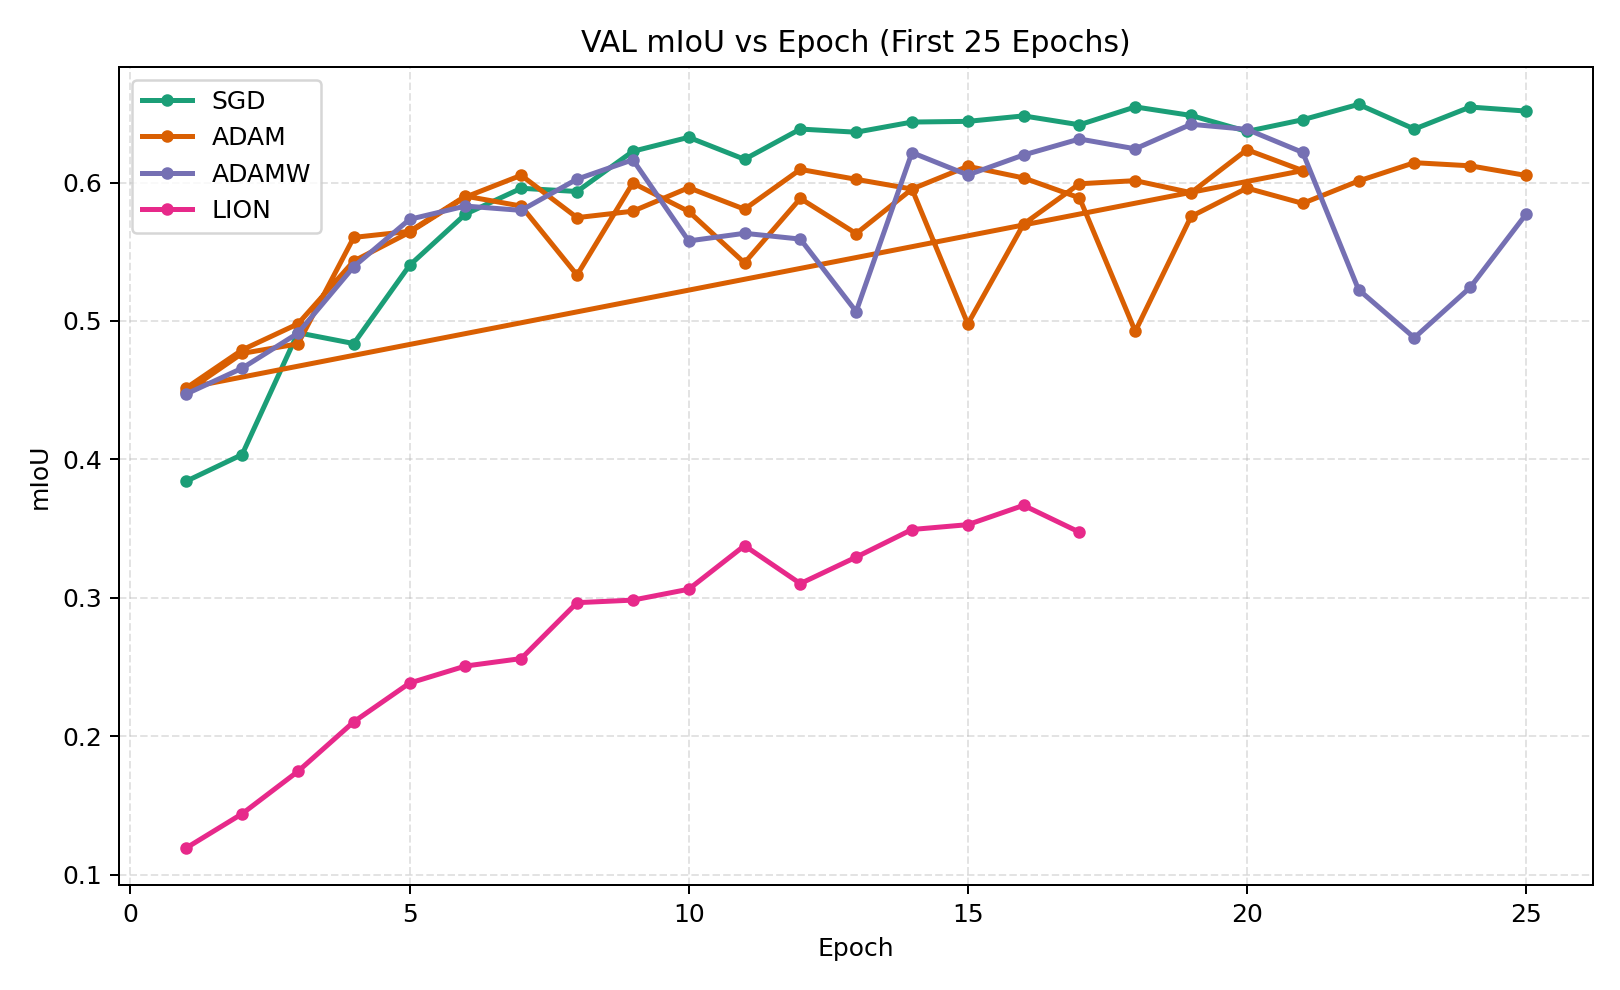
\includegraphics[width=\linewidth]{fig01_val_miou.png}
    \caption{Val mIoU}
\end{subfigure}\hfill
\begin{subfigure}[t]{0.32\linewidth}
    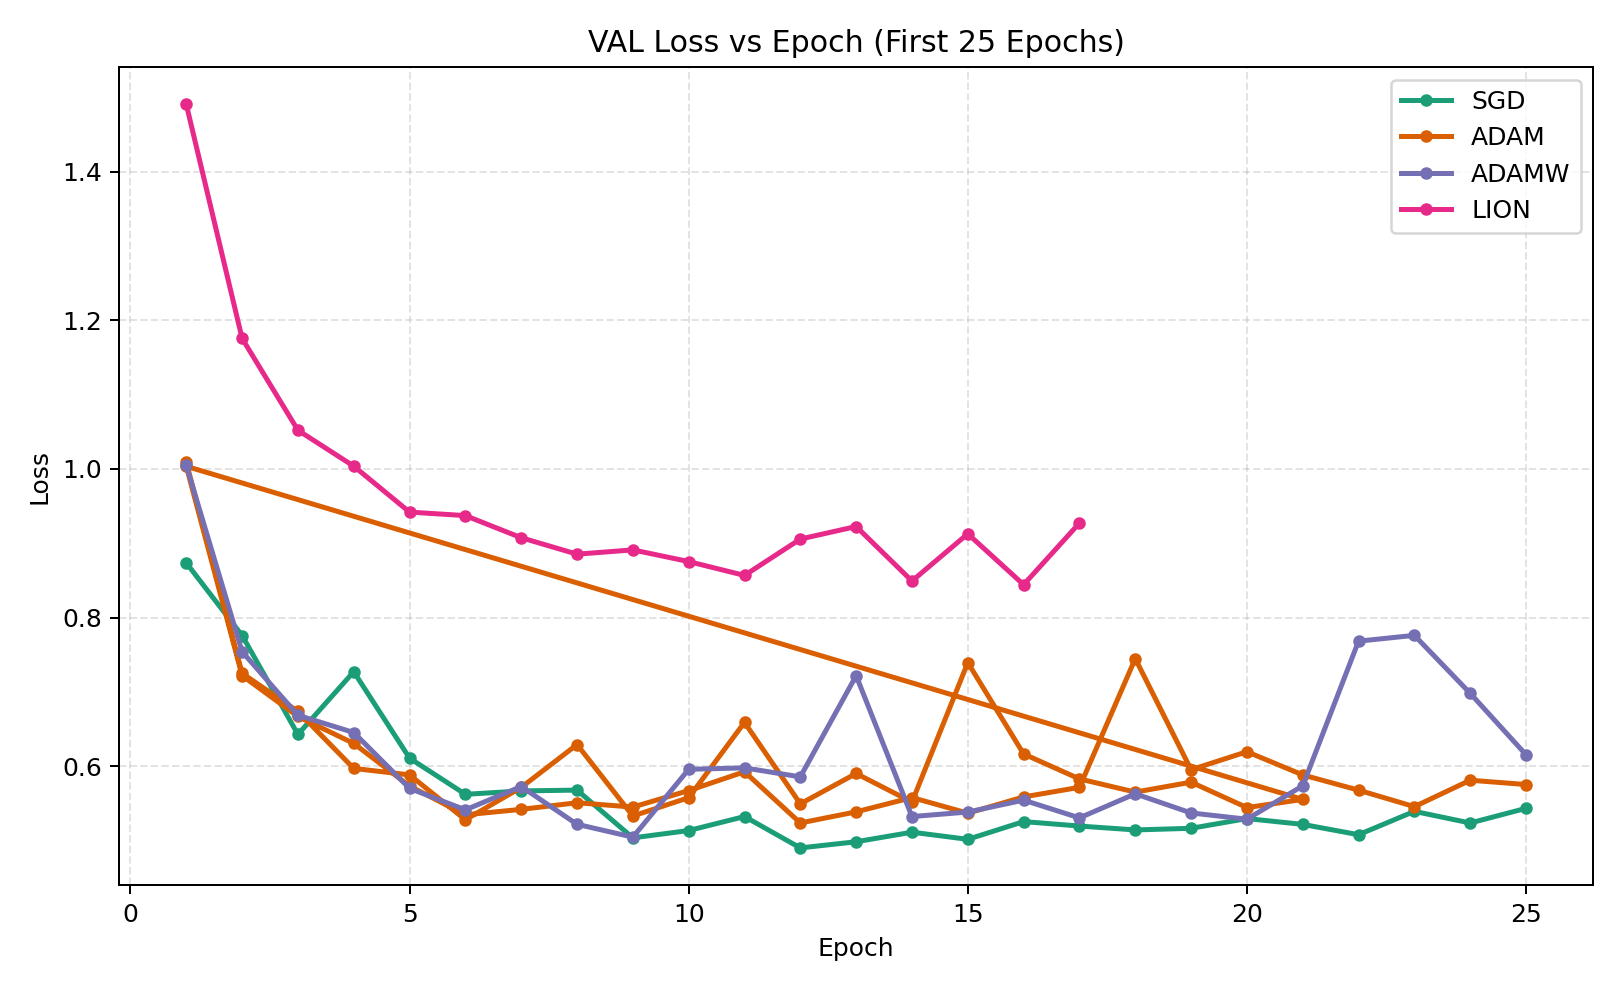
\includegraphics[width=\linewidth]{fig02_val_loss.png}
    \caption{Val loss}
\end{subfigure}\hfill
\begin{subfigure}[t]{0.32\linewidth}
    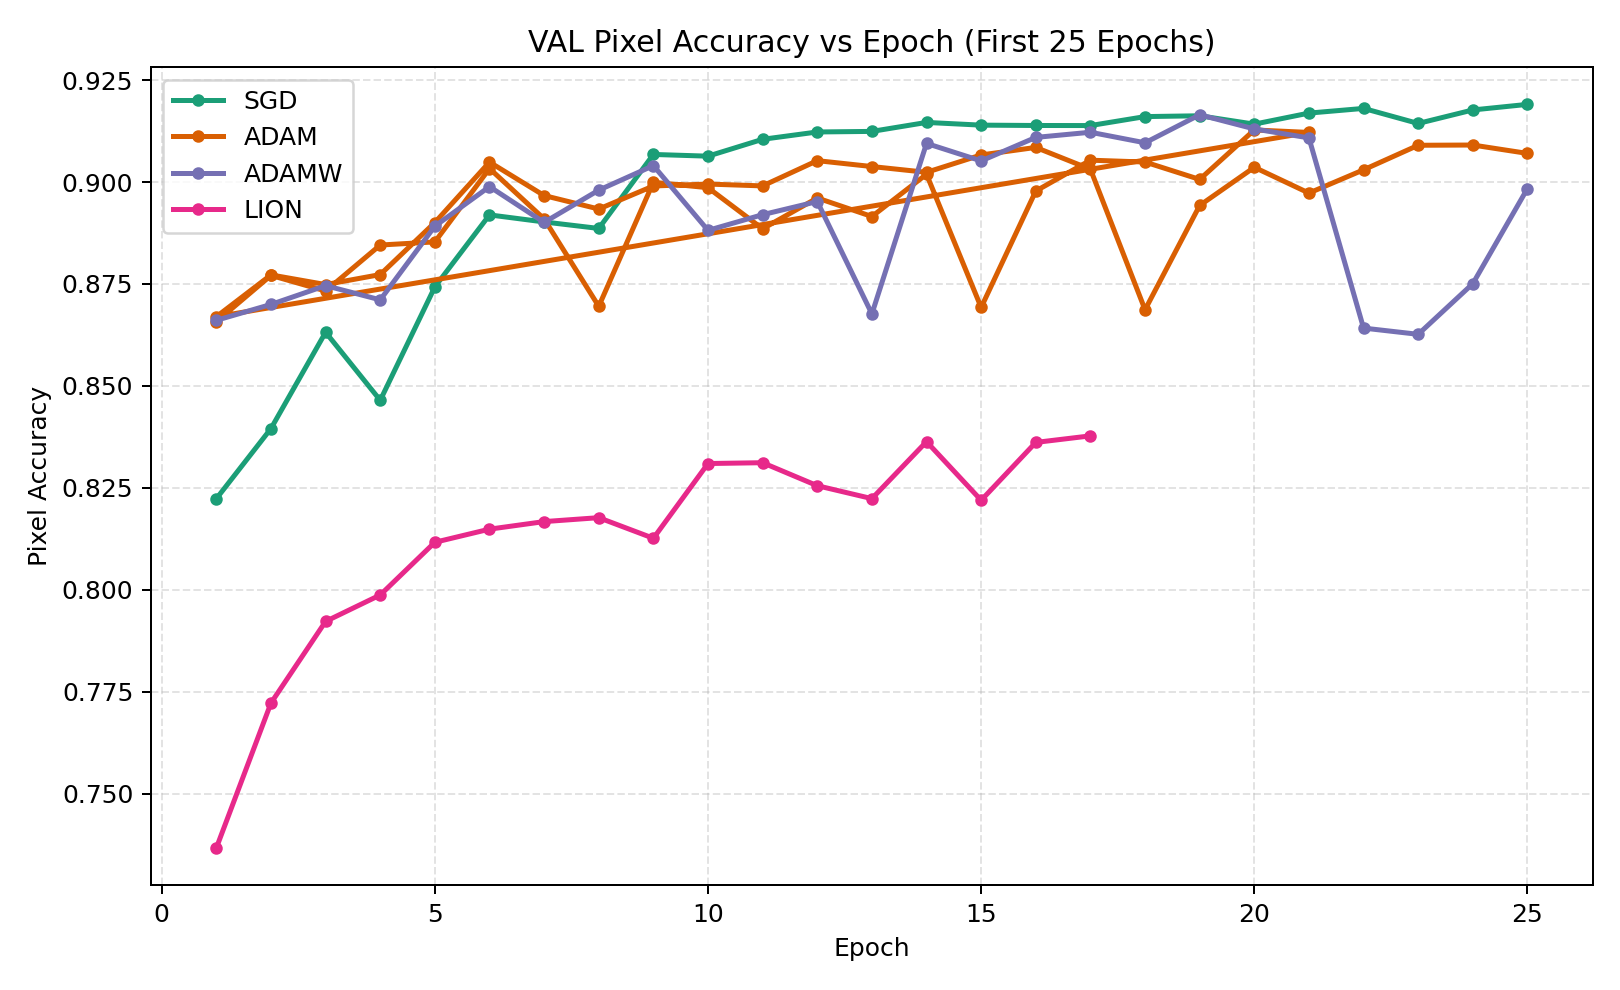
\includegraphics[width=\linewidth]{fig03_val_pixel_accuracy.png}
    \caption{Val pixel acc.}
\end{subfigure}

\vspace{-0.55em}
\begin{subfigure}[t]{0.32\linewidth}
    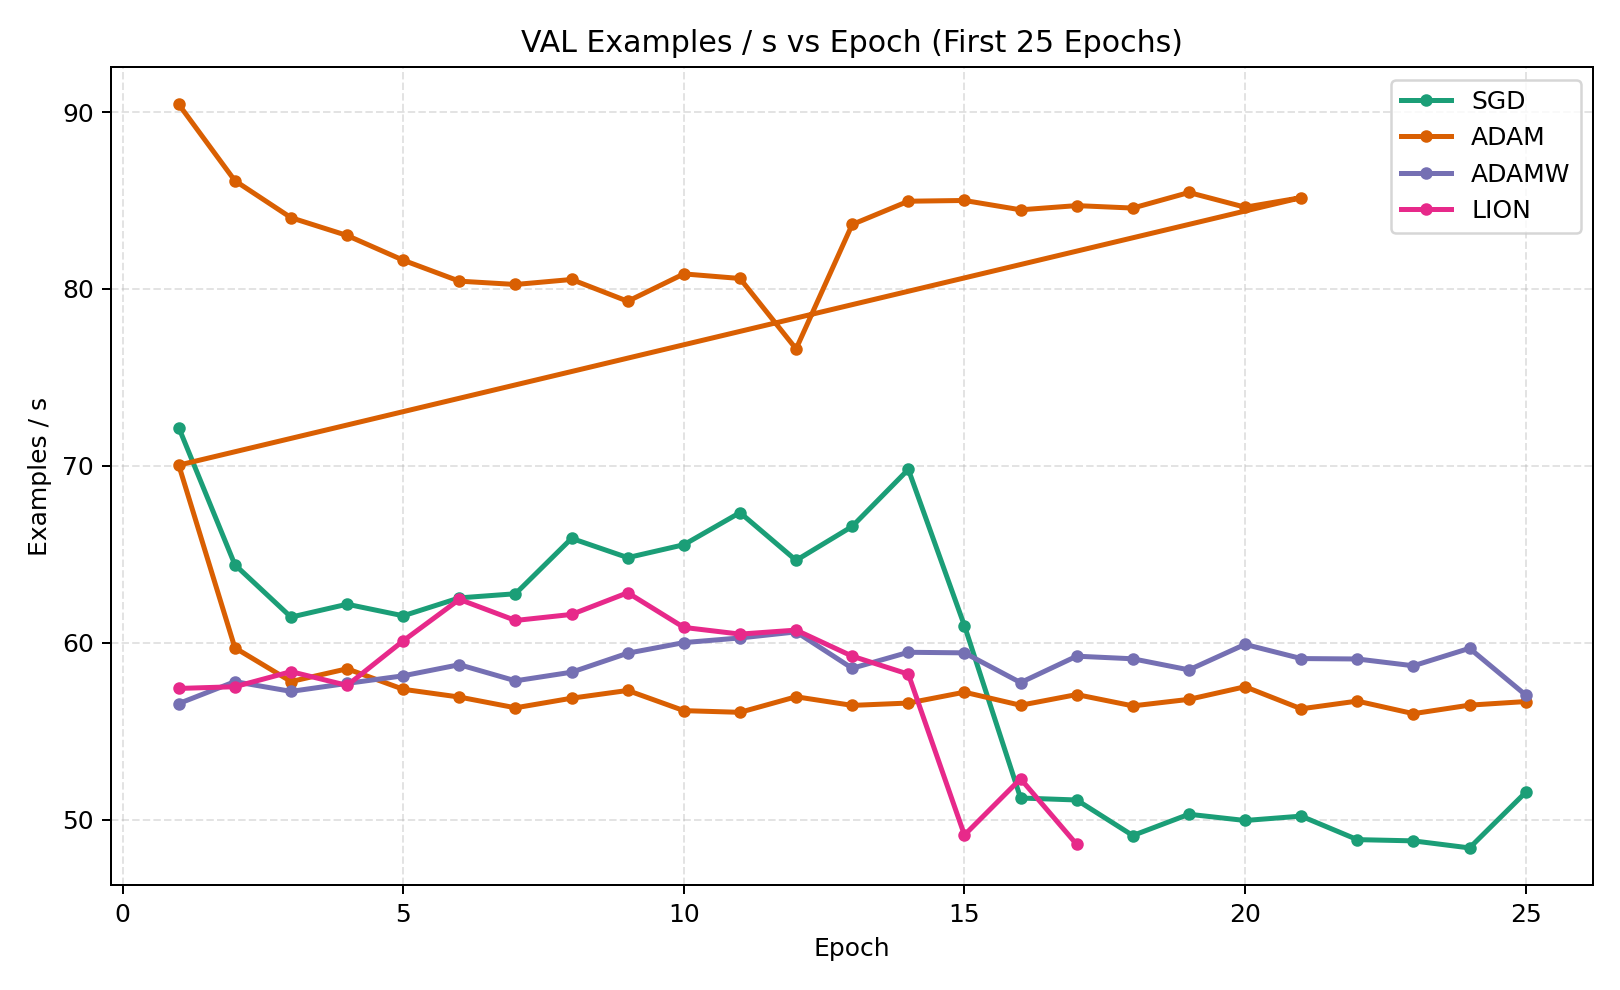
\includegraphics[width=\linewidth]{fig04_val_throughput.png}
    \caption{Val throughput}
\end{subfigure}\hfill
\begin{subfigure}[t]{0.32\linewidth}
    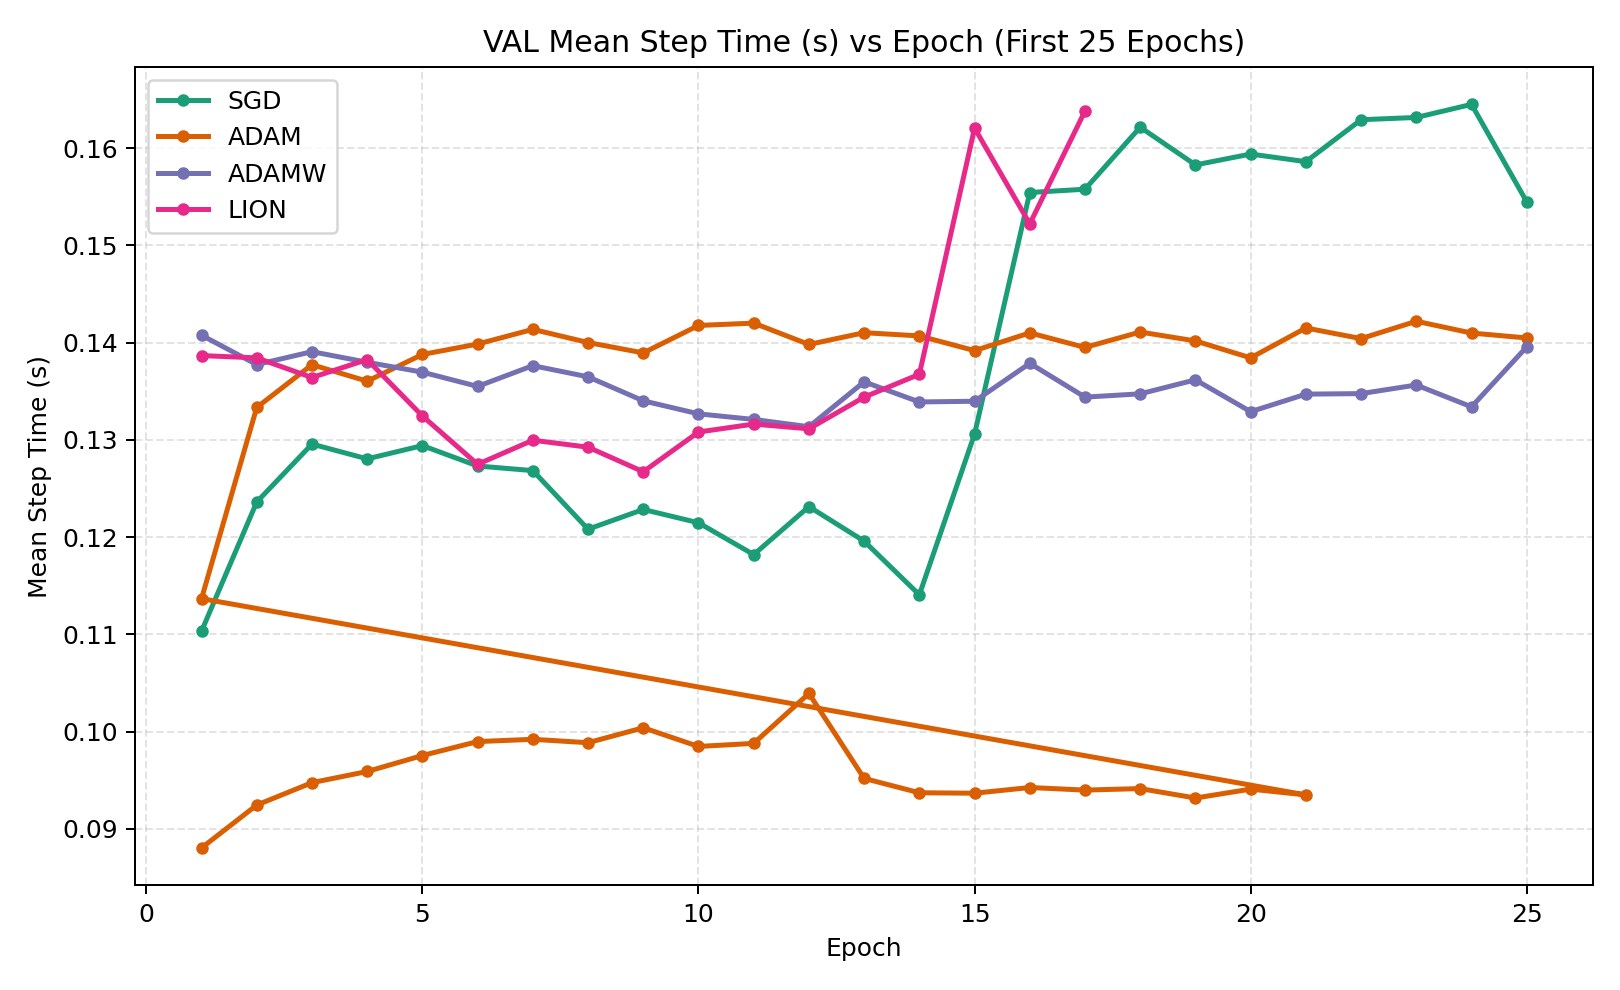
\includegraphics[width=\linewidth]{fig05_val_step_time.png}
    \caption{Val step time}
\end{subfigure}\hfill
\begin{subfigure}[t]{0.32\linewidth}
    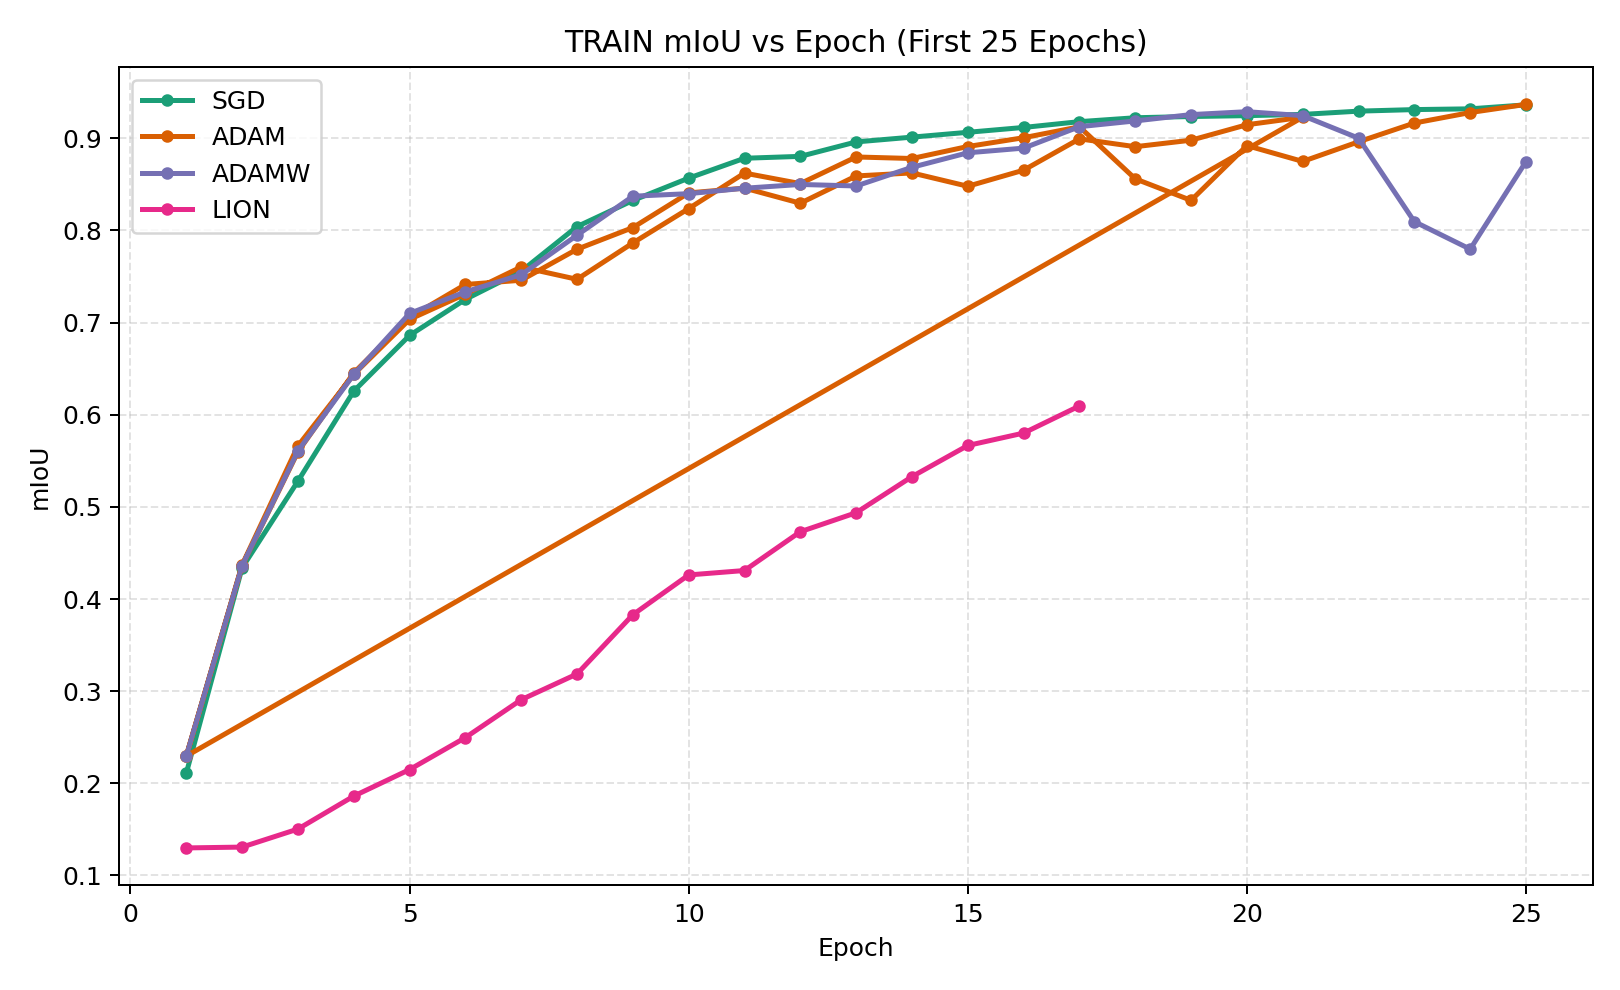
\includegraphics[width=\linewidth]{fig06_train_miou.png}
    \caption{Train mIoU}
\end{subfigure}
\caption{Validation quality metrics and the first training quality comparison.}
\end{figure}

\begin{figure}[H]
\centering
\begin{subfigure}[t]{0.32\linewidth}
    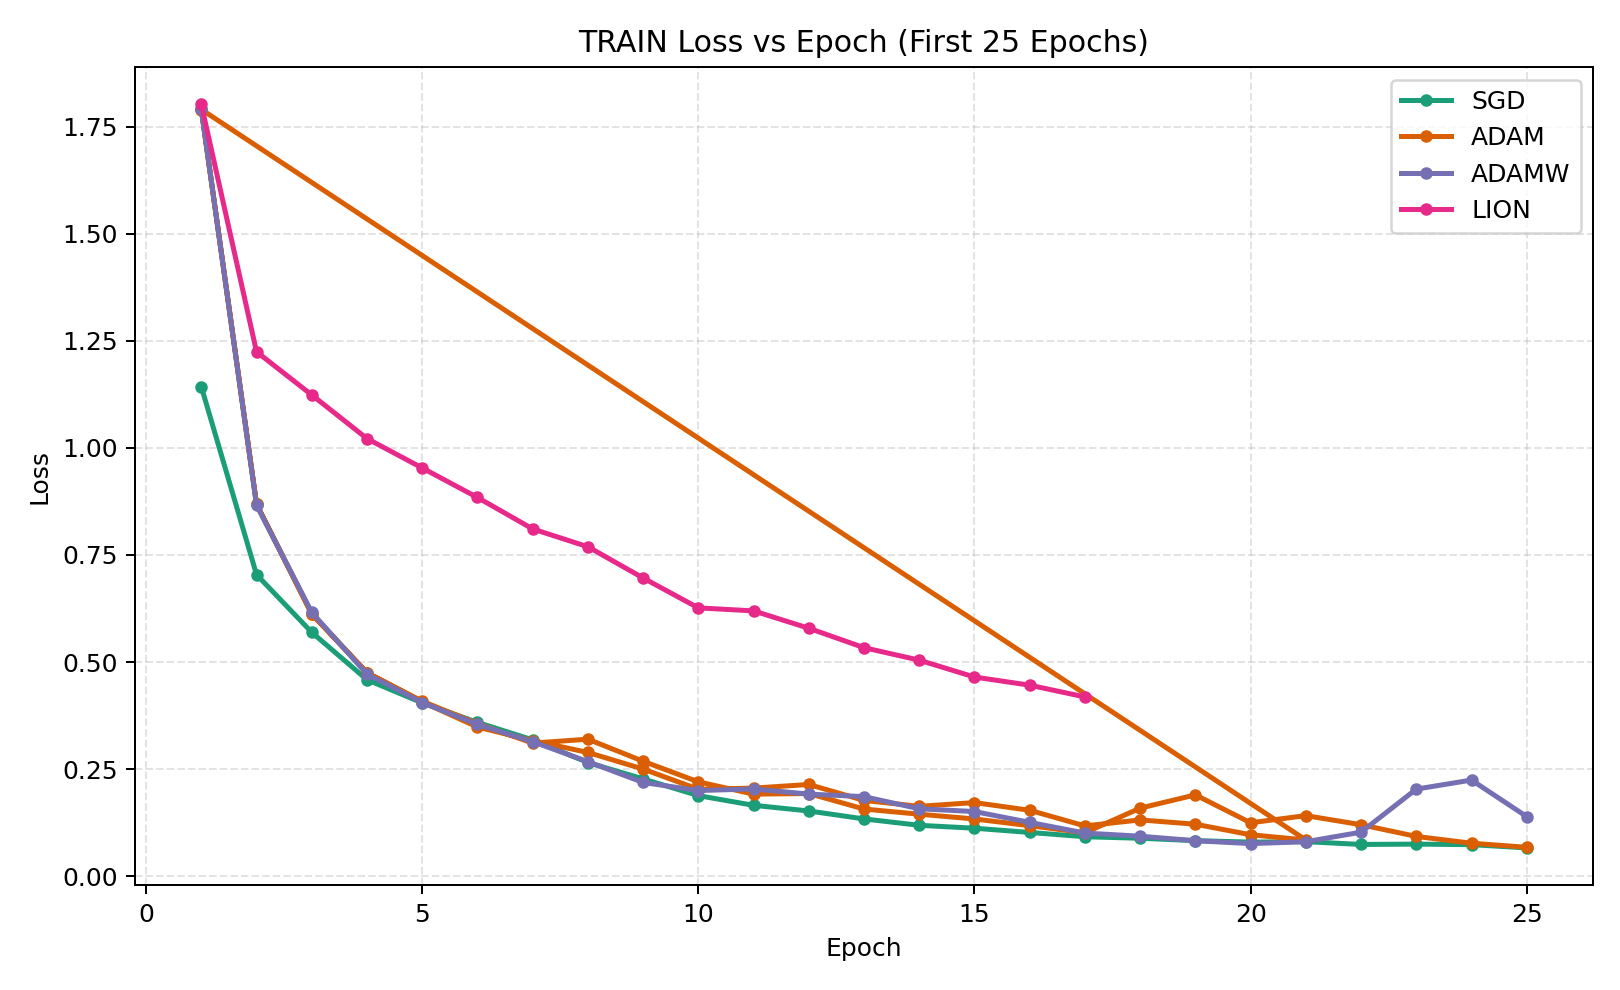
\includegraphics[width=\linewidth]{fig07_train_loss.png}
    \caption{Train loss}
\end{subfigure}\hfill
\begin{subfigure}[t]{0.32\linewidth}
    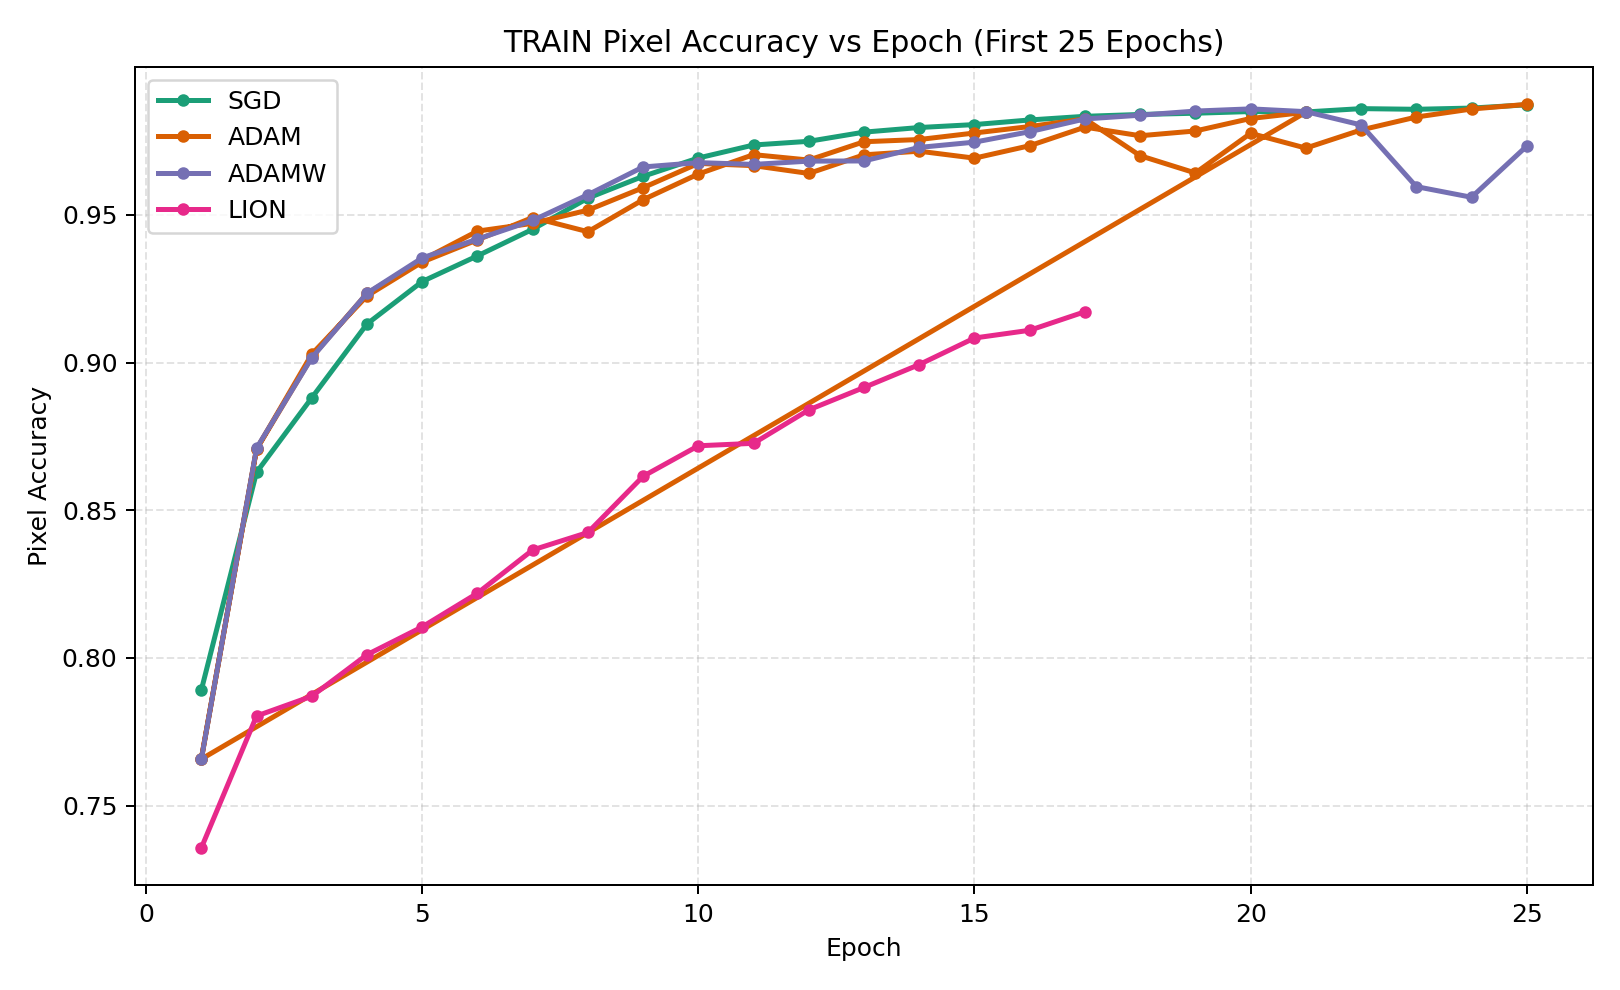
\includegraphics[width=\linewidth]{fig08_train_pixel_accuracy.png}
    \caption{Train pixel acc.}
\end{subfigure}\hfill
\begin{subfigure}[t]{0.32\linewidth}
    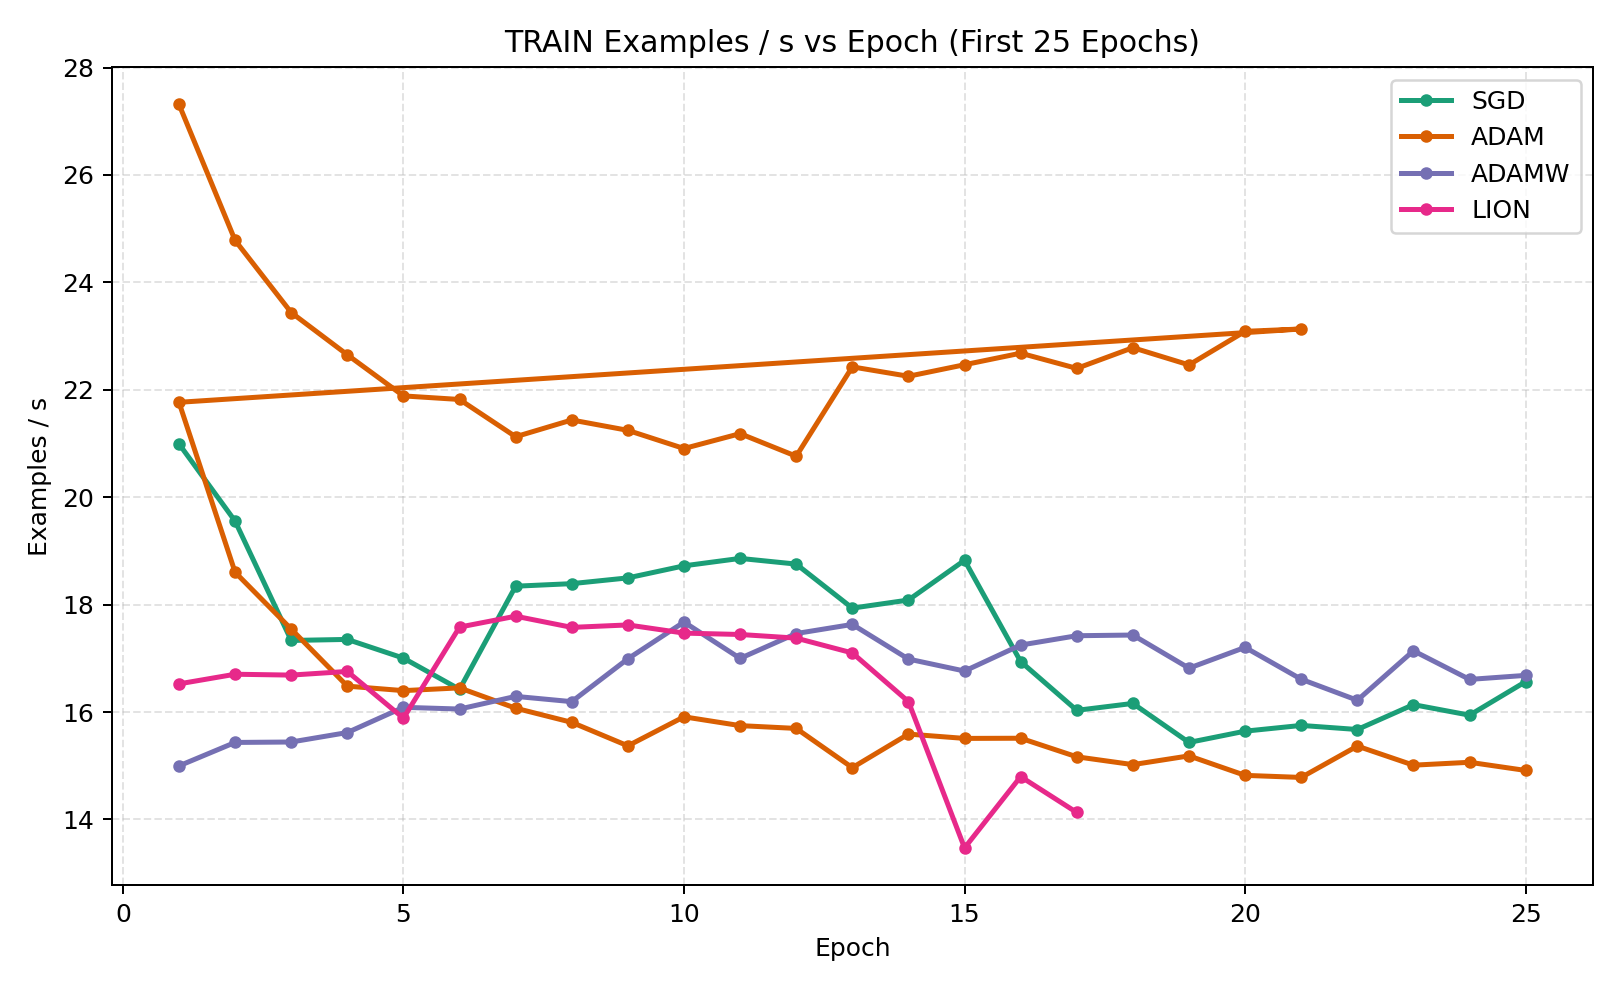
\includegraphics[width=\linewidth]{fig09_train_throughput.png}
    \caption{Train throughput}
\end{subfigure}

\vspace{-0.55em}
\begin{subfigure}[t]{0.32\linewidth}
    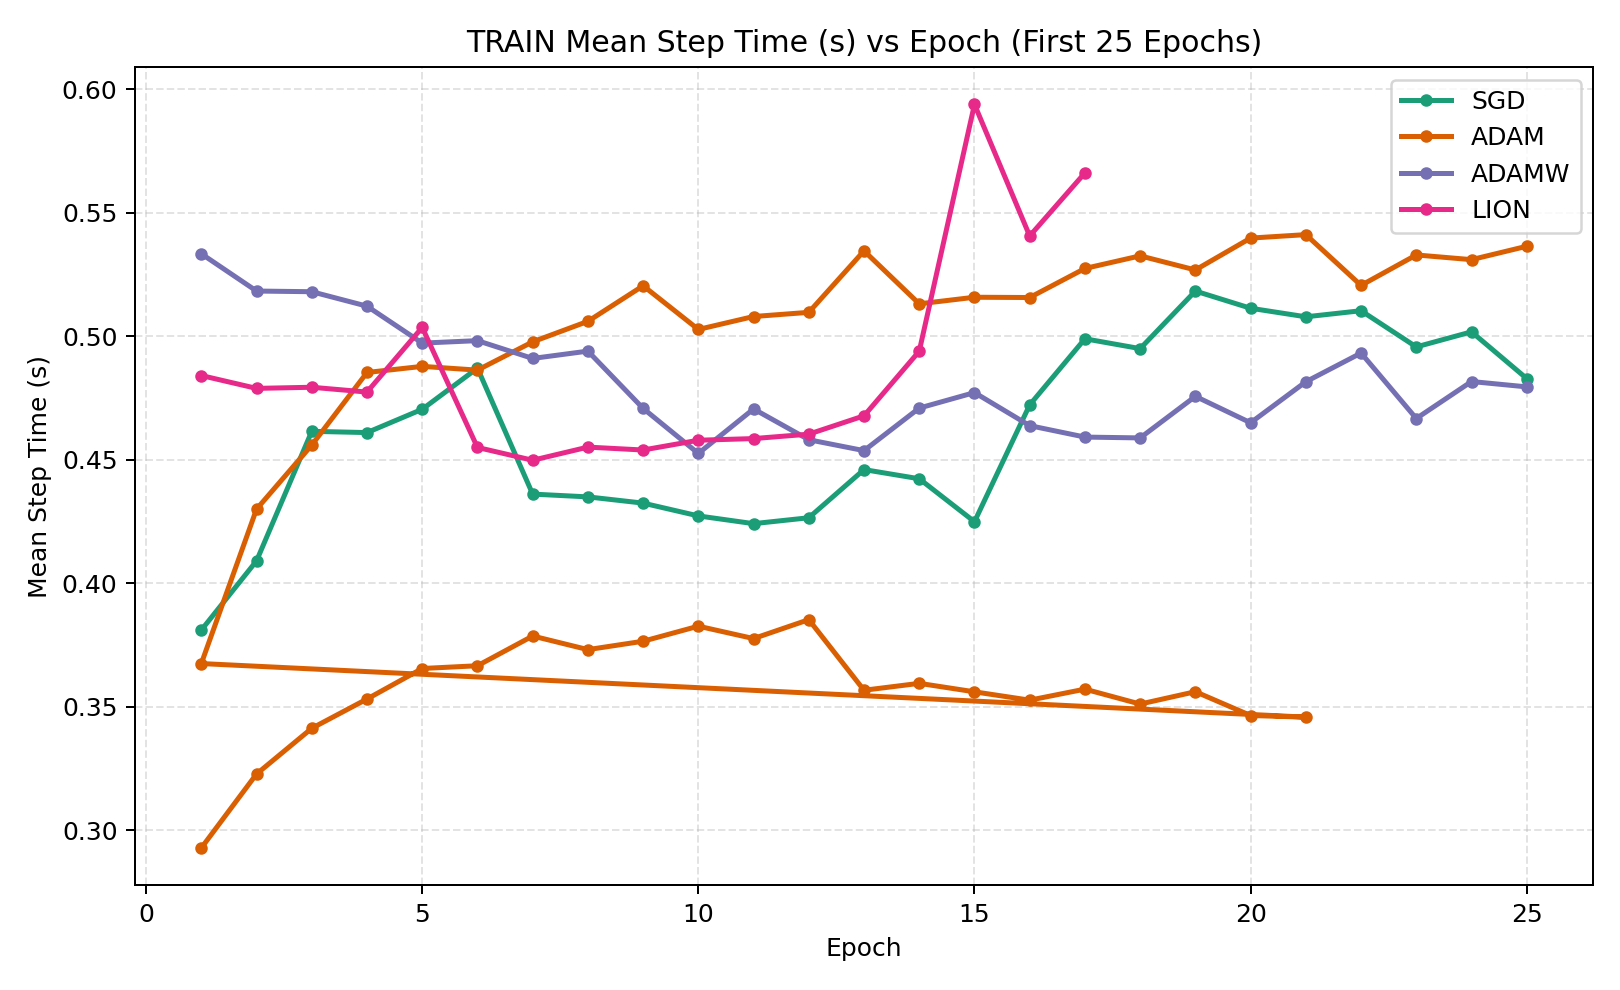
\includegraphics[width=\linewidth]{fig10_train_step_time.png}
    \caption{Train step time}
\end{subfigure}\hfill
\begin{subfigure}[t]{0.32\linewidth}
    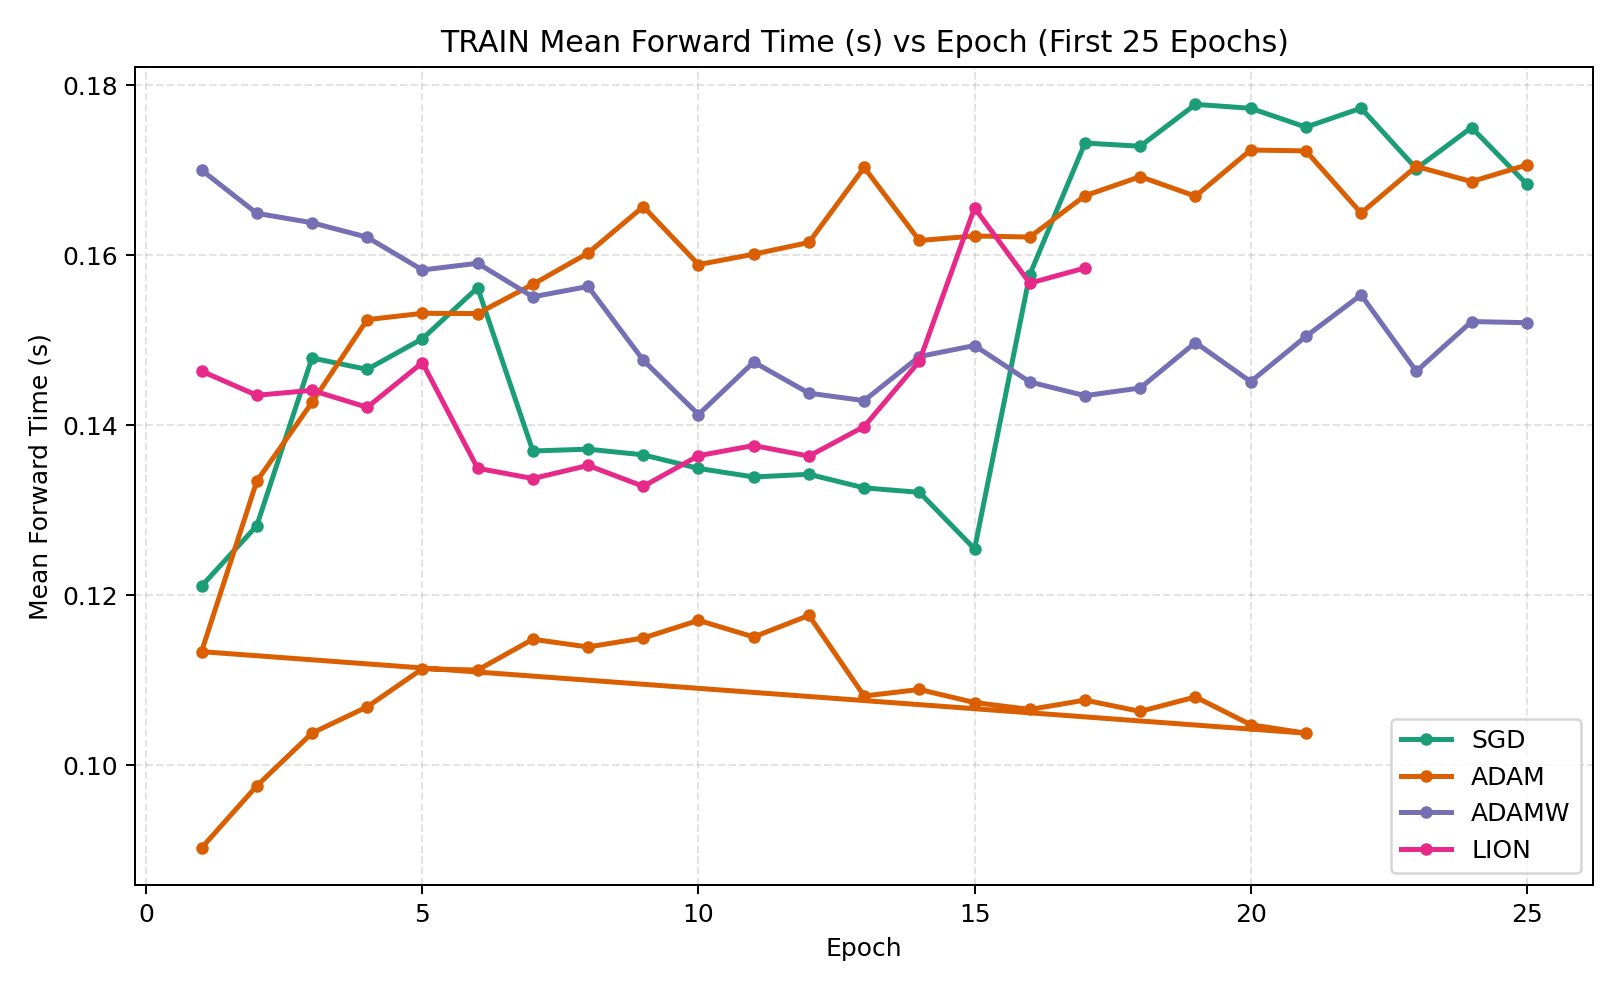
\includegraphics[width=\linewidth]{fig11_train_forward_time.png}
    \caption{Forward time}
\end{subfigure}\hfill
\begin{subfigure}[t]{0.32\linewidth}
    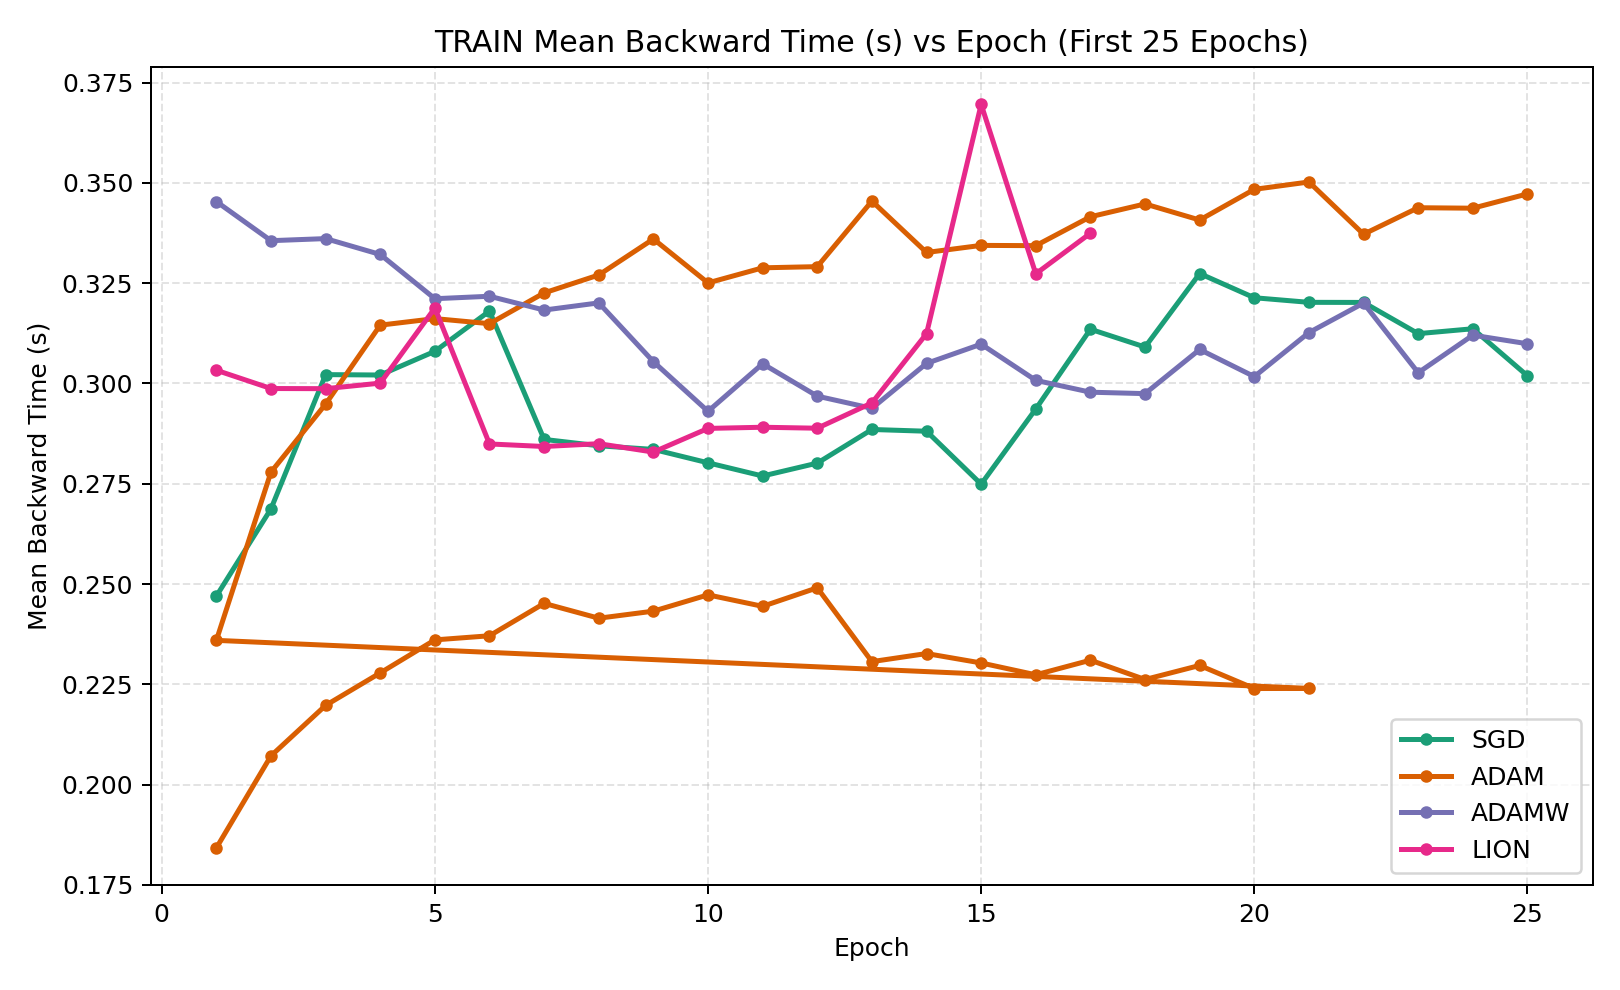
\includegraphics[width=\linewidth]{fig12_train_backward_time.png}
    \caption{Backward time}
\end{subfigure}
\caption{Training quality and efficiency metrics.}
\end{figure}

\begin{figure}[H]
\centering
\begin{subfigure}[t]{0.32\linewidth}
    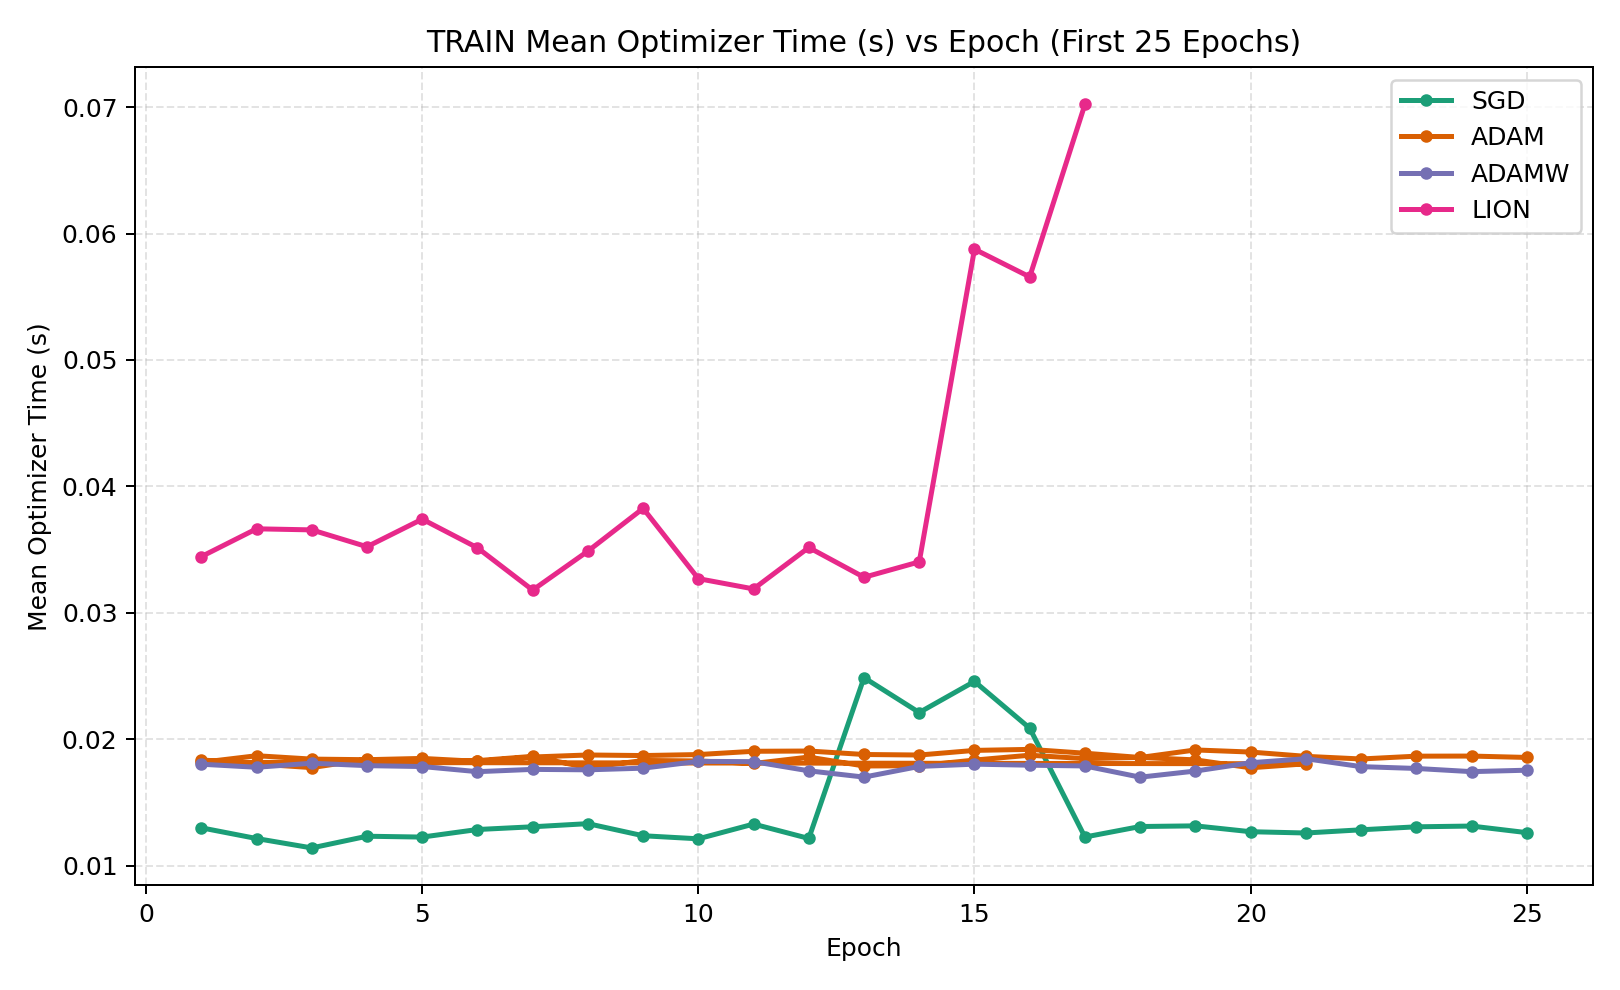
\includegraphics[width=\linewidth]{fig13_train_optimizer_time.png}
    \caption{Optimizer time}
\end{subfigure}\hfill
\begin{subfigure}[t]{0.32\linewidth}
    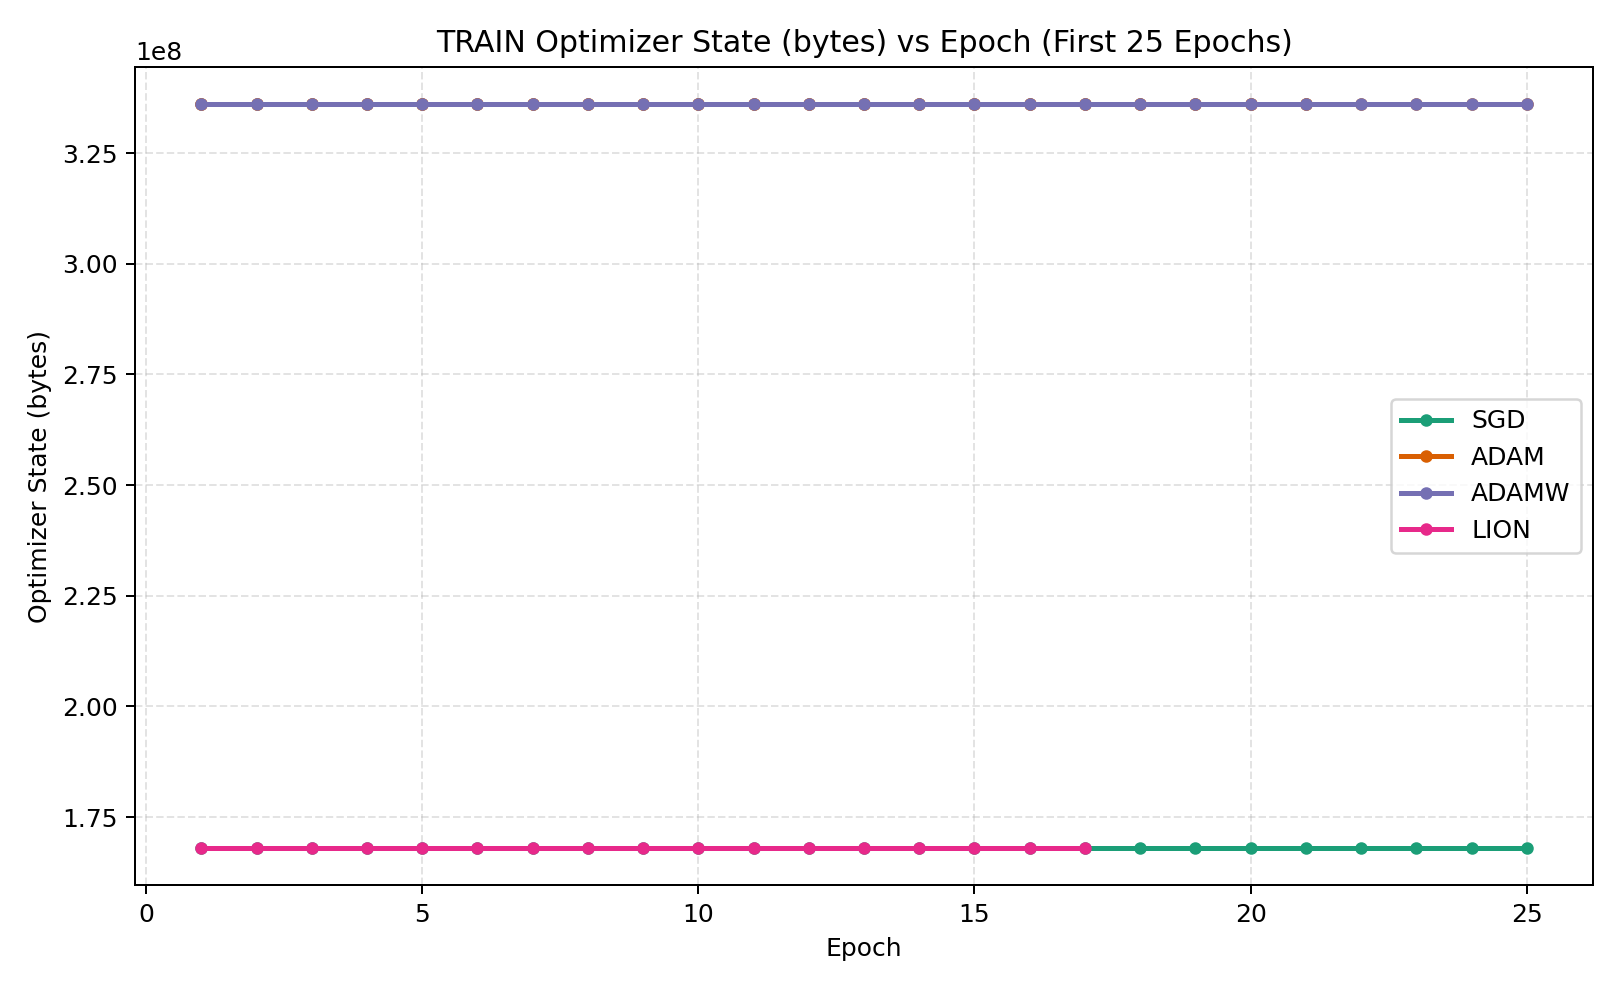
\includegraphics[width=\linewidth]{fig14_optimizer_state_bytes_curve.png}
    \caption{Optimizer state}
\end{subfigure}\hfill
\begin{subfigure}[t]{0.32\linewidth}
    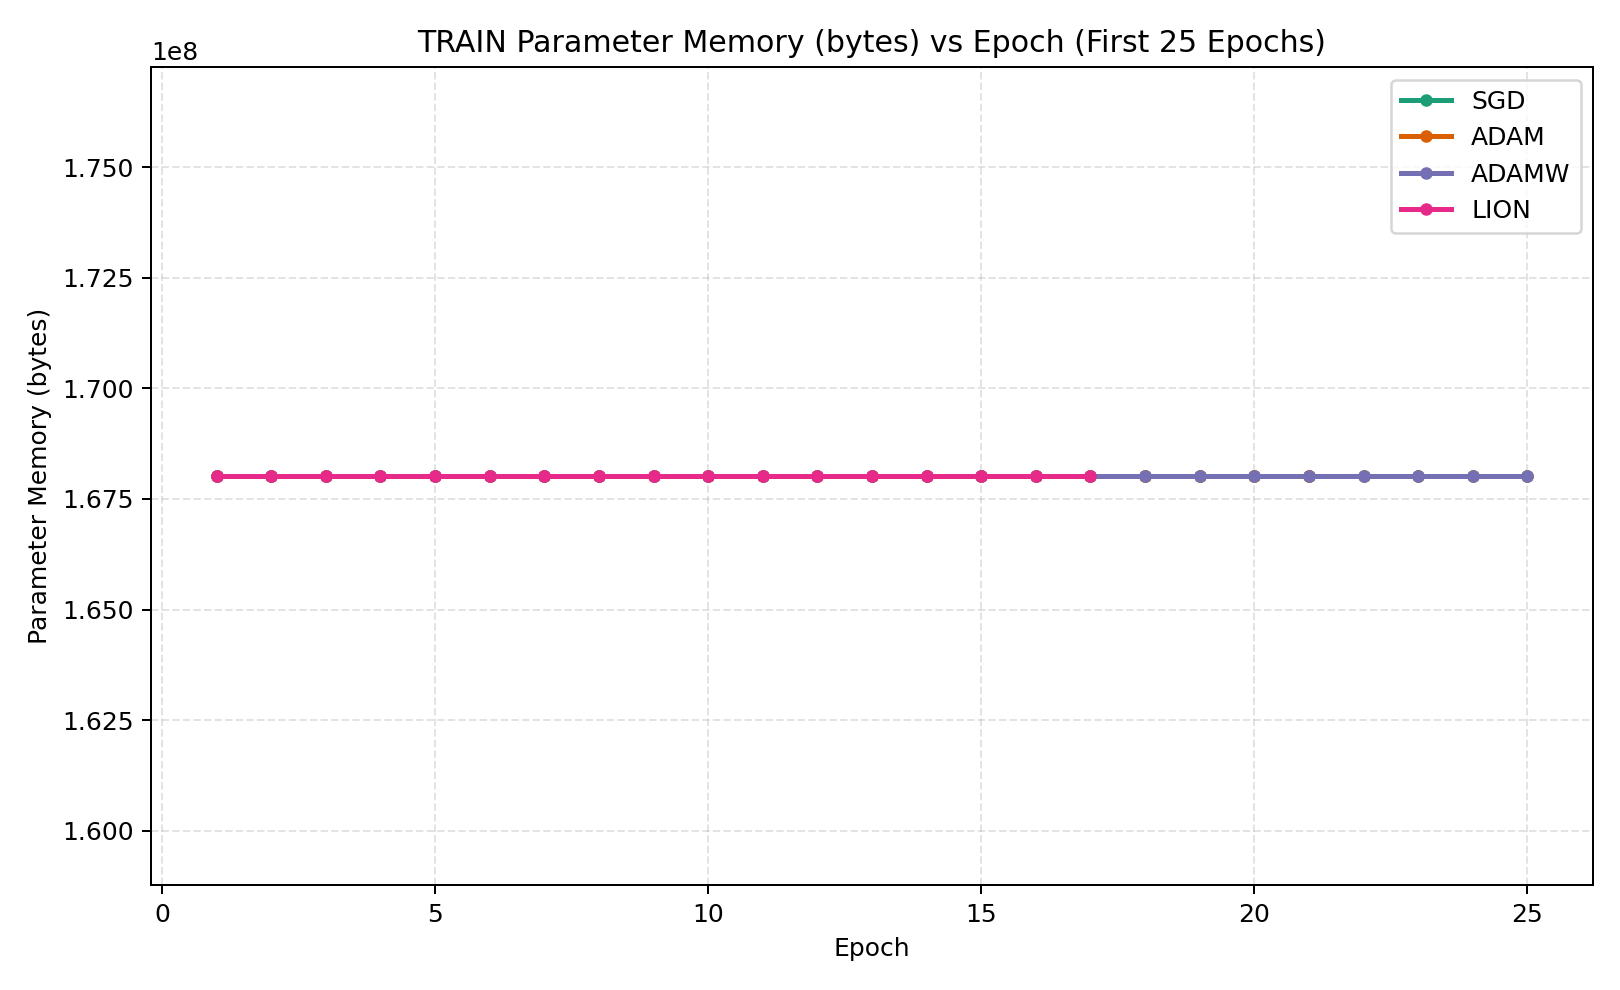
\includegraphics[width=\linewidth]{fig15_parameter_bytes_curve.png}
    \caption{Parameter bytes}
\end{subfigure}

\vspace{-0.55em}
\begin{subfigure}[t]{0.32\linewidth}
    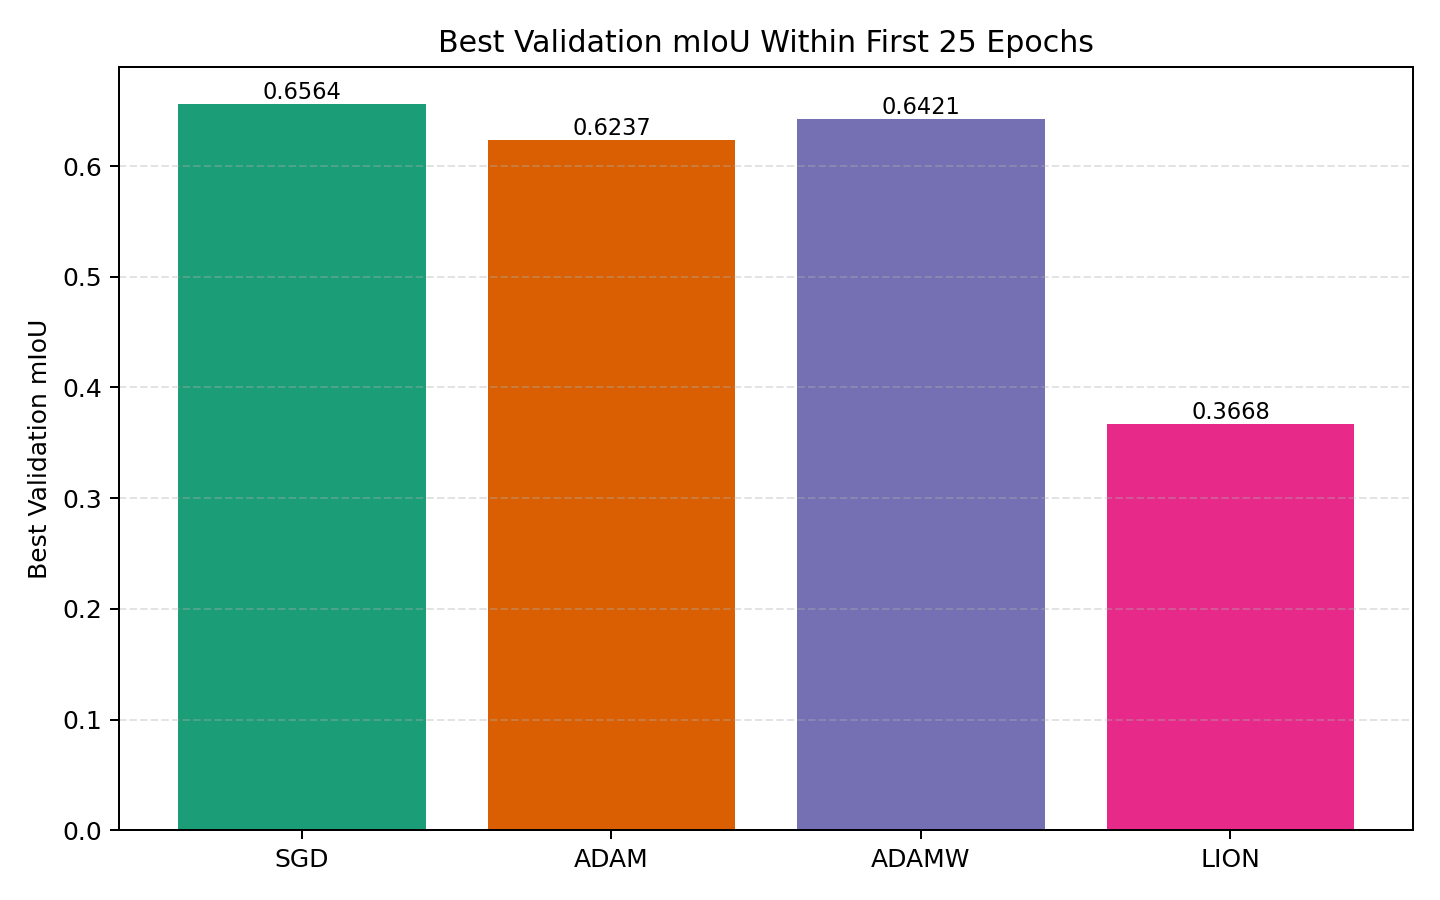
\includegraphics[width=\linewidth]{fig16_best_val_miou_bar.png}
    \caption{Best val mIoU}
\end{subfigure}\hfill
\begin{subfigure}[t]{0.32\linewidth}
    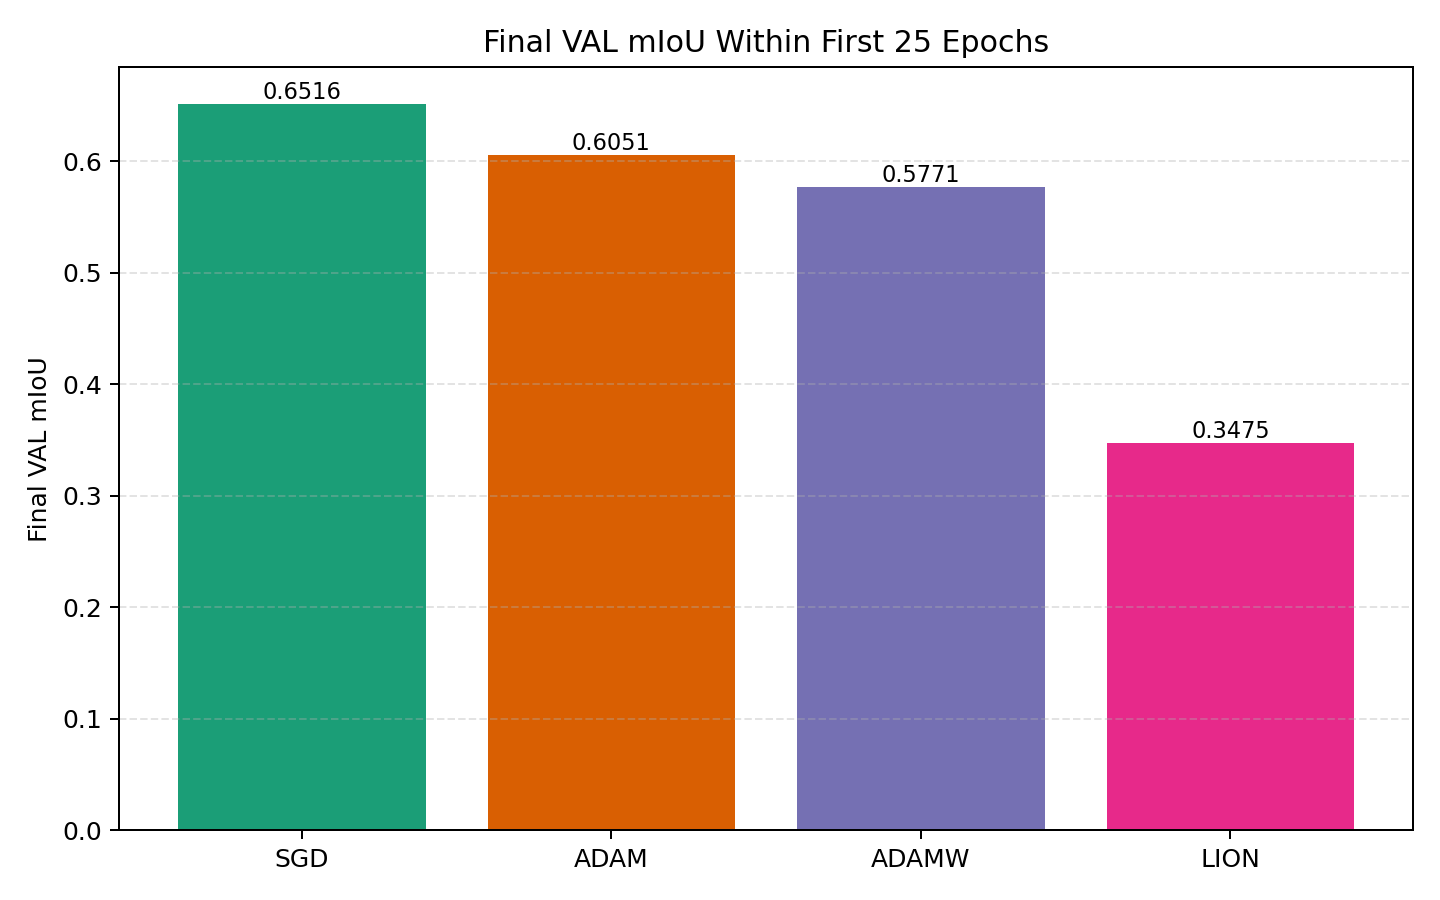
\includegraphics[width=\linewidth]{fig17_final_val_miou_bar.png}
    \caption{Final val mIoU}
\end{subfigure}\hfill
\begin{subfigure}[t]{0.32\linewidth}
    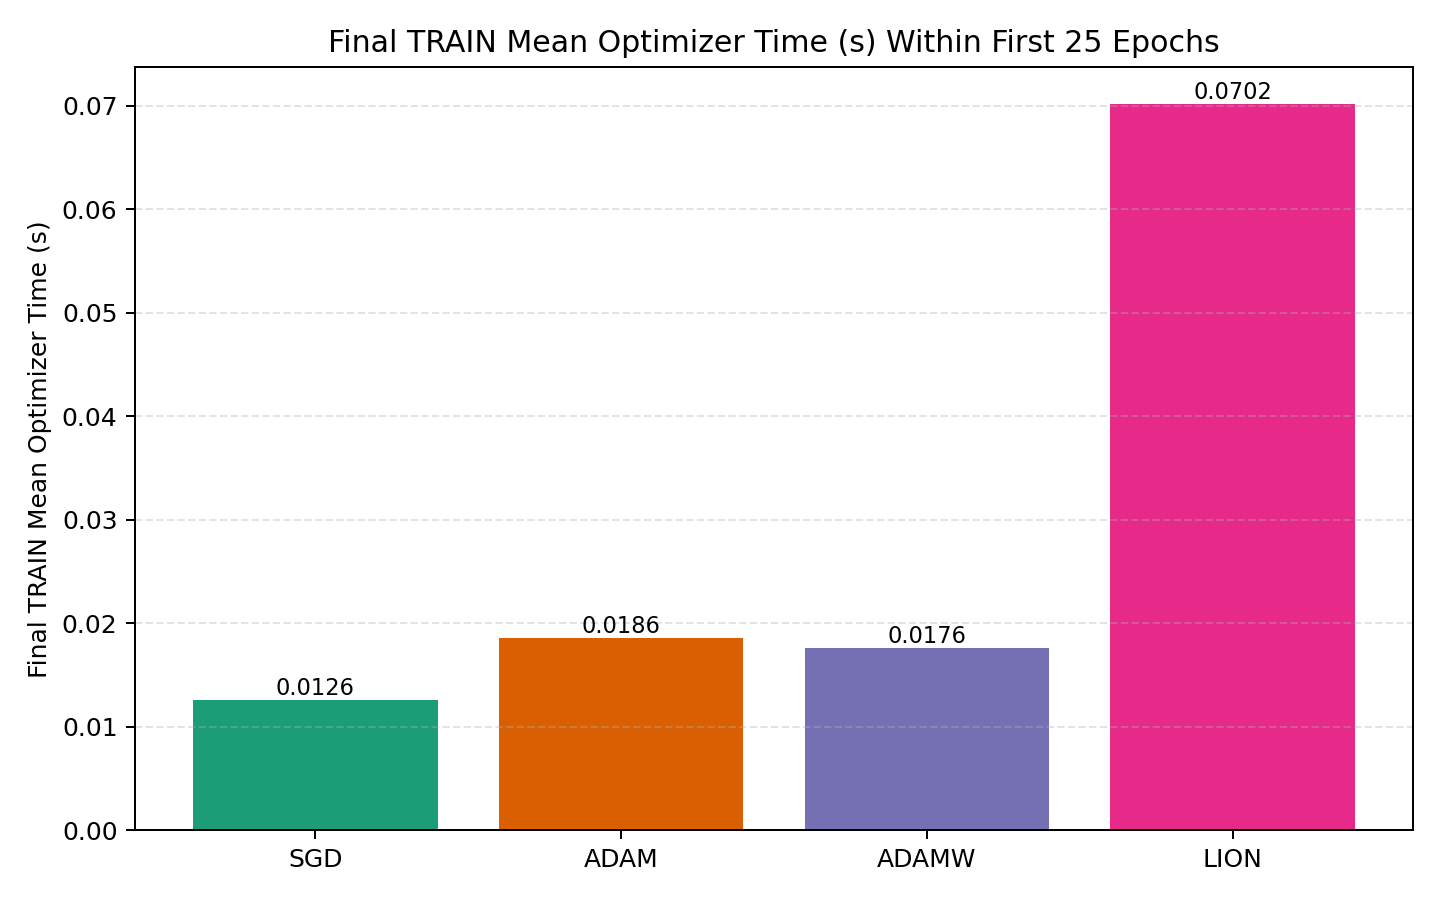
\includegraphics[width=\linewidth]{fig18_final_optimizer_time_bar.png}
    \caption{Final optimizer time}
\end{subfigure}
\caption{Optimizer overhead, memory, and summary bars.}
\end{figure}

\begin{figure}[H]
\centering
\begin{subfigure}[t]{0.495\linewidth}
    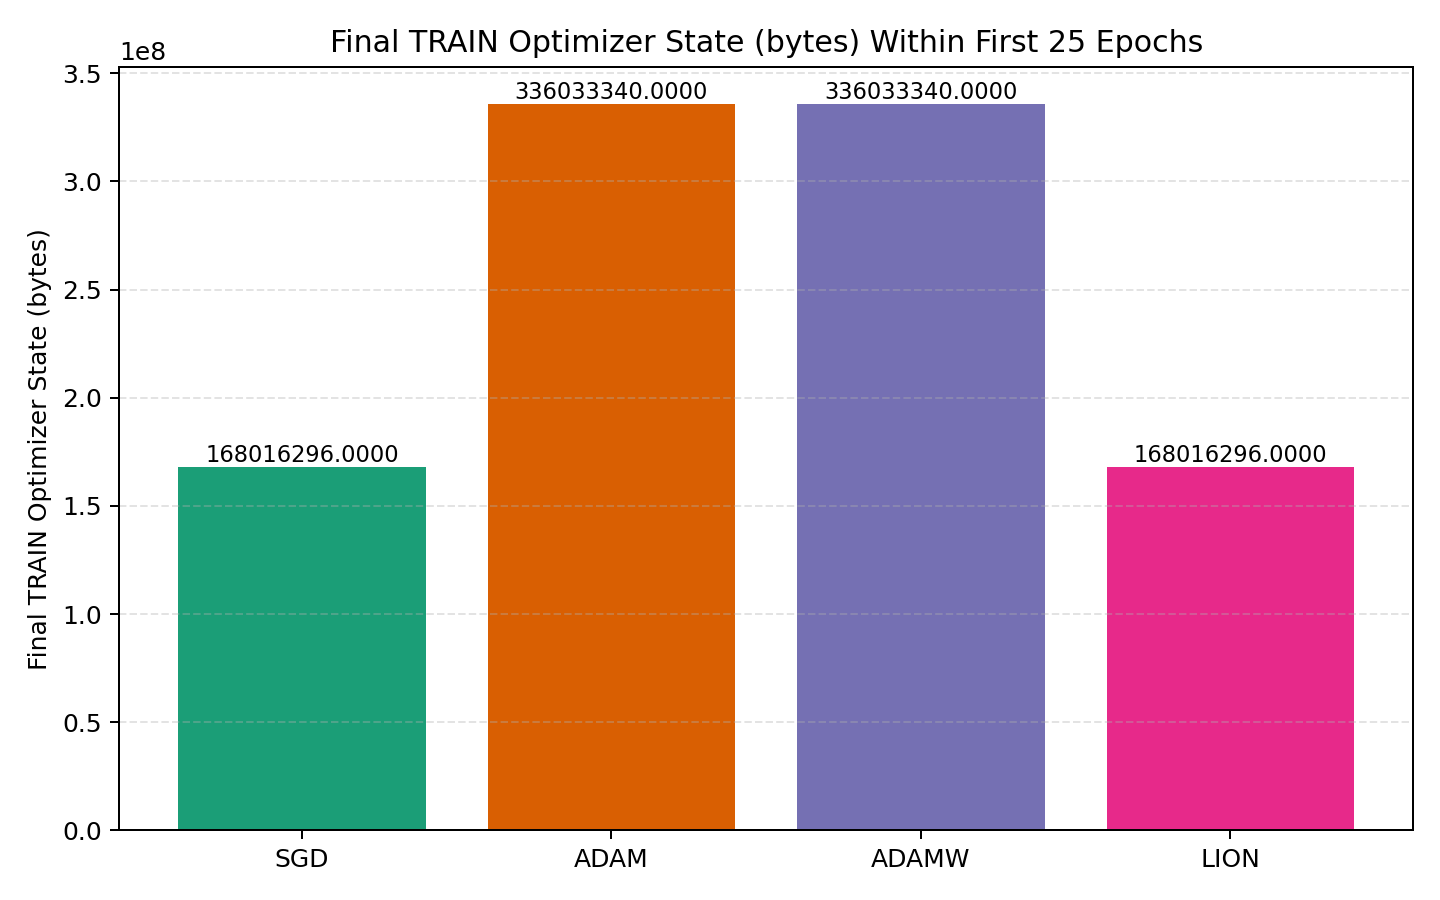
\includegraphics[width=\linewidth]{fig19_final_optimizer_state_bar.png}
    \caption{Final optimizer state memory}
\end{subfigure}\hfill
\begin{subfigure}[t]{0.495\linewidth}
    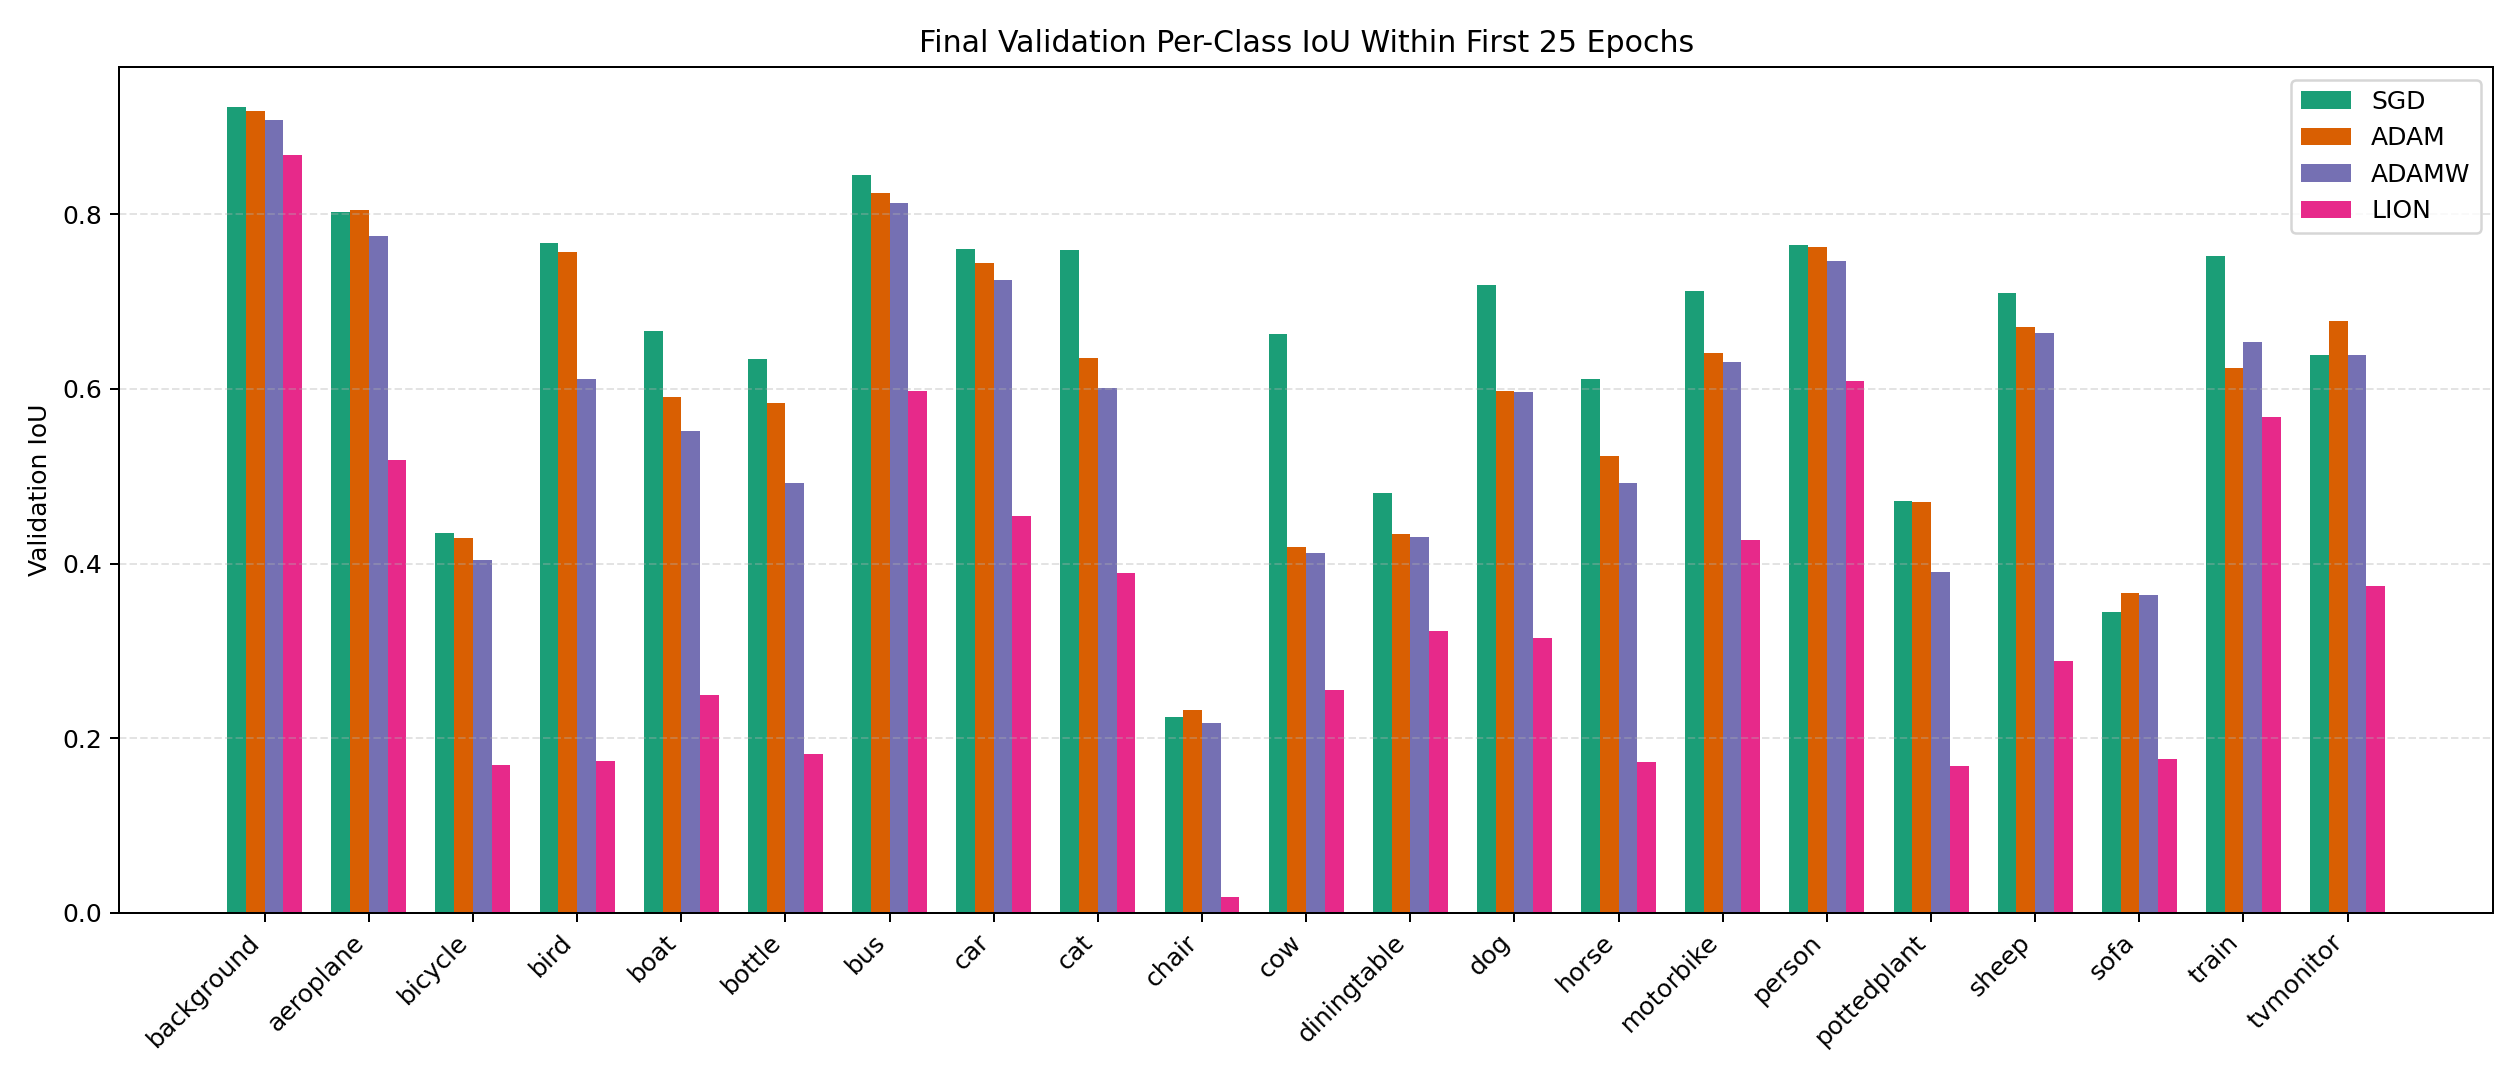
\includegraphics[width=\linewidth]{fig20_final_per_class_iou.png}
    \caption{Final per-class validation IoU}
\end{subfigure}
\caption{Final memory summary and class-wise segmentation comparison.}
\end{figure}

\section{Future Work and Conclusion}
Our next step is to extend the benchmark from Pascal VOC to \textbf{ADE20K} and a text classification task such as \textbf{AG News} so that the analysis covers multiple tasks, as intended in the original proposal. This will allow us to evaluate stability across tasks by examining whether Lion, AdamW, SGD with momentum, and RMSProp exhibit consistent convergence behavior, sensitivity to hyperparameters, and variance across repeated runs in both vision and language settings. Alongside predictive performance, we will continue the systems efficiency analysis by measuring runtime per training step, total training time, and peak memory usage for each optimizer, so that the final comparison captures both accuracy and practical computational tradeoffs. By adding these tasks, the project will move from a single-dataset study toward a broader empirical analysis of optimizer behavior across different training settings and application domains.

At the current stage, when all optimizers are compared under the same 25-epoch budget, \textbf{SGD} provides the best overall performance on Pascal VOC segmentation with DeepLabV3-ResNet50. \textbf{AdamW} is the strongest adaptive baseline and remains competitive, while \textbf{Adam} trails both SGD and AdamW. \textbf{Lion} has not yet shown a quality or efficiency advantage in this setting. The Pascal VOC benchmark therefore serves as a strong first step in a broader optimizer-comparison project that we plan to continue on richer segmentation datasets and across multiple task domains.

\end{document}
